%%%%%%%%%%%%%%%%%%%%%%%%%%%%%%%%%%%%%%%%%%%%%%%%%%%%%%%%%%%%%%%%%%%%%%%%%%%%%%%
%
% Evaluation
% 
%%%%%%%%%%%%%%%%%%%%%%%%%%%%%%%%%%%%%%%%%%%%%%%%%%%%%%%%%%%%%%%%%%%%%%%%%%%%%%%


\chapter{Results and Discussion}
\label{sec:results}

The work of \citet{zhou1999vortex} is replicated in this thesis study. The characteristics of an elastically mounted circular cylinder suspended in a fluid domain is studied. The cylinder is free to oscillate in x and y direction, so two-Dimensional study is conducted. According to \citet{williamson1996vortex}, the upper limit of Reynolds number (Re) where the vortex shedding from a circular cylinder is still two-dimensional and the wake is laminar can reach 200. In the current study a laminar flow is considered with $Re=200$ which is the same as that of \citet{zhou1999vortex}. The inlet flow velocity is set to $U_\infty = 1 \frac{m}{s}$, the fluid density is considered as $\rho = 1 \frac{kg}{m^3}$ and the flow viscosity is calculated to be $\mu=\frac{1}{200} Pa s$. These factors are tabulated as shown in \ref{table:4.1}. 

\begin{table}[H]
 \centering
	\begin{tabular}{|c|c|}
		\hline 
		Parameter & Value\tabularnewline
		\hline 
		Re & 200\tabularnewline
		\hline 
		U {[}m/s{]} & 1\tabularnewline
		\hline 
		D {[}m{]} & 1\tabularnewline
		\hline 
		$\mu$ {[}Pa s{]} & 1/200\tabularnewline
		\hline 
		$\rho$ {[}$\frac{kg}{m^{3}}${]} & 	1\tabularnewline
		\hline 
	\end{tabular}
\caption{Laminar flow properties and the diameter of the cylinder considered}
\label{table:4.1}
\end{table}

\section{Computational Grid}

A 2-D \textit{O-Grid} mesh is generated around the cylinder. The first cell is placed at a distance of $0.0025*D$ from the cylinder wall. The growth rate is set to $1.05$, a total of $240x200 (r x \theta)$ control volumes are generated for the domain. The distance from the cylinder to the outer boundary is considered to be $15*D$. Two blocks are generated which is further split into 4 blocks each, along the radial axis for grid parallelization. Since this is a two-dimensional analysis, span-wise grid is not refined or resolved. A time step size of 0.001 s is considered for the current study. 

The selected time step leads to a maximum Courant number of around 0.4. The maximum Courant number $(C_{max})$ is a dimensionless number which is obtained
by evaluating the Courant-Friedrichs-Lewy condition or CFL condition which can be written as   
\begin{equation}
C = \frac{u \Delta t}{\Delta x} \leq C_max
\label{eqn:4.1} 
\end{equation}

where C is the dimensionless Courant number in every time-step.

The generated grid, inlet and outlet boundary patches considered are highlighted in the figure \ref{fig:4.1}.
\begin{figure}[h]
%\centering
	\begin{minipage}[t]{4cm}
		\fbox{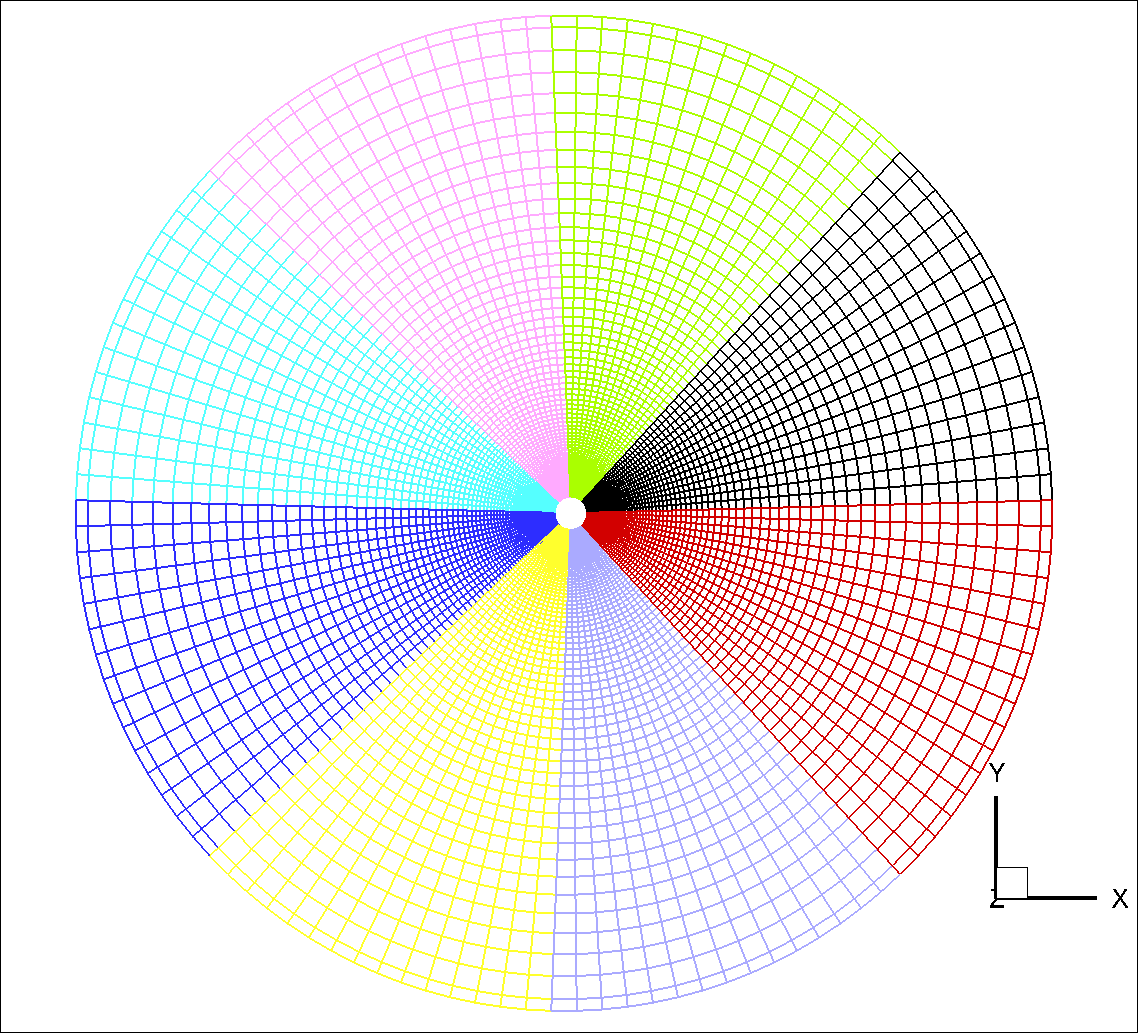
\includegraphics[height=2.65in]{grid}}
%		\caption{Grids colored by blocks of parallelization}
	\end{minipage}
	\hspace{4cm}
	\begin{minipage}[t]{4cm}
%		\centering
		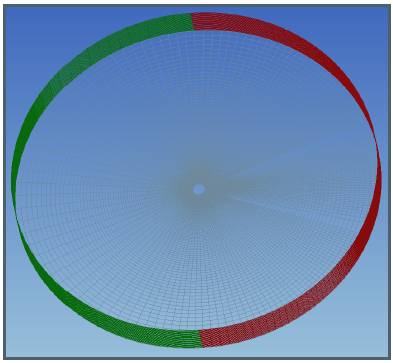
\includegraphics[height=2.65in]{grid_inout}
%		\caption{Grids colored by blocks of parallelization}
	\end{minipage}
\caption{Left: Grids colored by blocks of parallelization; Right: Grid highlighted with inlet (Green) and outlet(Red) patches}
\label{fig:4.1}
\end{figure}

This same mesh has been used for all the simulations in the current study.

\section{Results of flow analysis}
Initially a flow analysis for a flow around a fixed cylinder is conducted. In FASTEST-3D, convective boundary conditions are implemented for outlet boundaries in order to overcome the short-comings of zero-gradient outlet. The convective boundary conditions are implemented by solving explicitly a convective transport equation. The convective transport equation can be written in the form
\[ \frac {\partial U_i}{\partial t} + \frac{\partial U^c_j
  U_i}{\partial x_j} = 0 ~; 
\]
which equals to 
\[ \frac {\partial U_i}{\partial t} + U^c \frac{\partial U_i}{\partial
  x} + V^c \frac{\partial U_i}{\partial y} + W^c \frac{\partial
  U_i}{\partial z}   = 0 ~,
\]

where $ U^c_j = ( U^c V^c W^c )^T $ is the velocity vector of the
convection.\\

The boundary conditions used for the simulation is tabulated in \ref{table:4.2}. The simulation is run for a total of 200,000 time-steps, i.e. for a physical time of 200s. 

\begin{table} [H]
\centering
	\begin{tabular}{|c|c|}
	\hline 
	Boundary  & Boundary condition \tabularnewline
	\hline 
	\multirow{2}{*}{Inlet} & Velocity Inlet \tabularnewline
	\cline{2-2} 
	 & $U_{x}$ = 1 m/s \tabularnewline
	\hline 
	\multirow{2}{*}{Outlet} & Convective boundary \tabularnewline
	\cline{2-2} 
	 & $U^{c}$ = 1\tabularnewline
	\hline 
	\end{tabular}
\caption{Boundary conditions considered for the simulation}
\label{table:4.2}
\end{table}

In the figure \ref{fig:4.2} the instantaneous velocity field behind the cylinder is presented. In can be observed that right behind the cylinder the vortices has maximum energy and as these vortices travel further down-stream the energy dissipates. By the time the vortices reaches the limit of the domain all the energy has been dissipated and vortices vanishes. The alternating vortex shedding can also be
observed from the instantaneous pressure contour in figure \ref{fig:4.3}. The vortex pattern in the wake composes of negative and positive staggered vortices, that is commonly referred to as \textit{Karman vortex street}. The shed vortices from the cylinder follows almost identical path downstream.  

%\begin{figure}[h]
%%\centering
%	\begin{minipage}[t]{4cm}
%		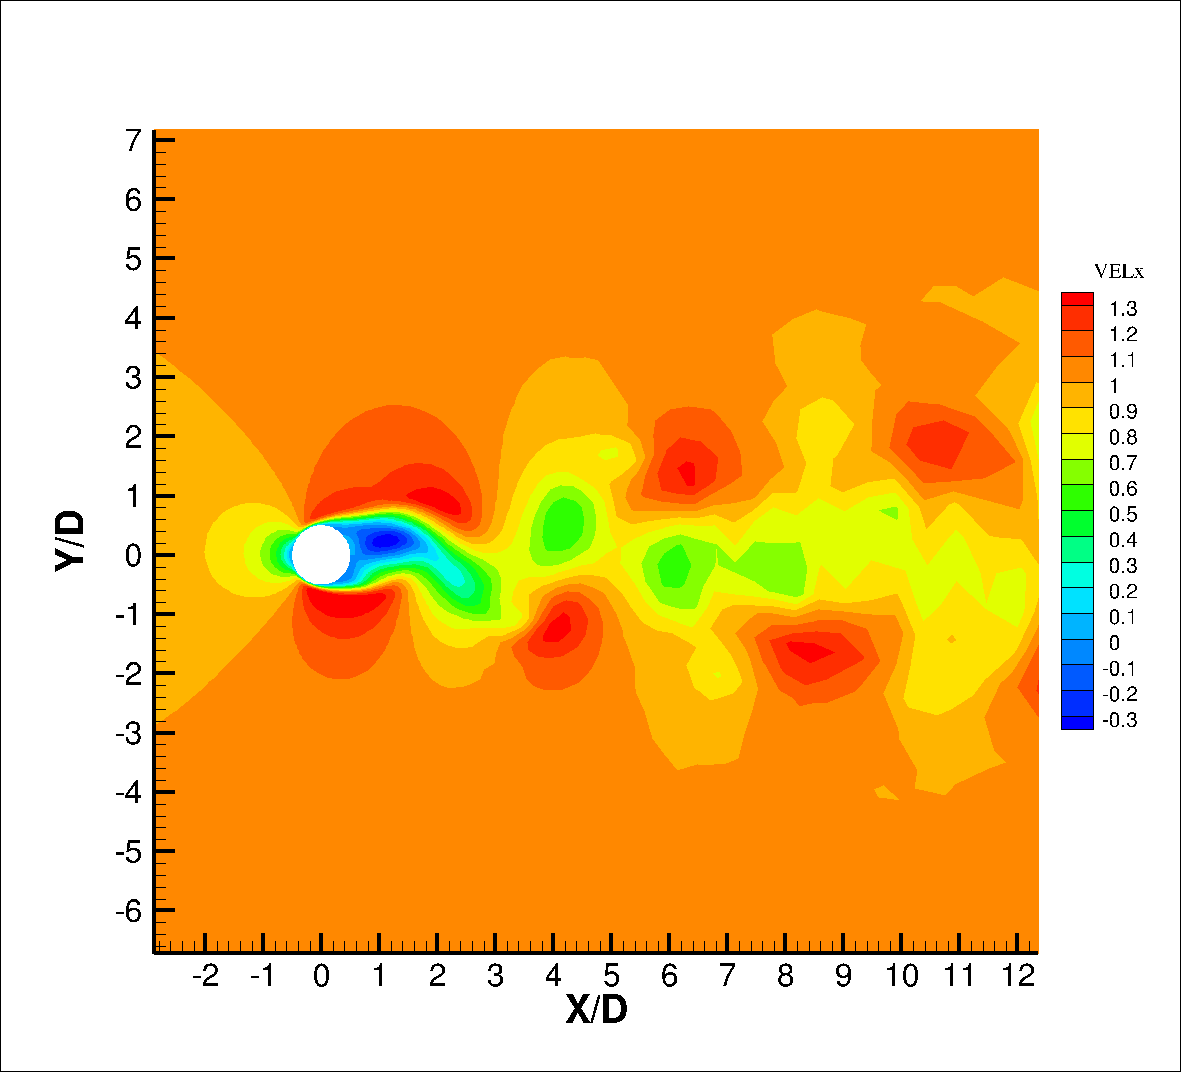
\includegraphics[height=2.6in]{Vx_181s}
%		\caption{t=181s}
%	\end{minipage}
%	\hspace{4cm}
%	\begin{minipage}[t]{4cm}
%%		\centering
%		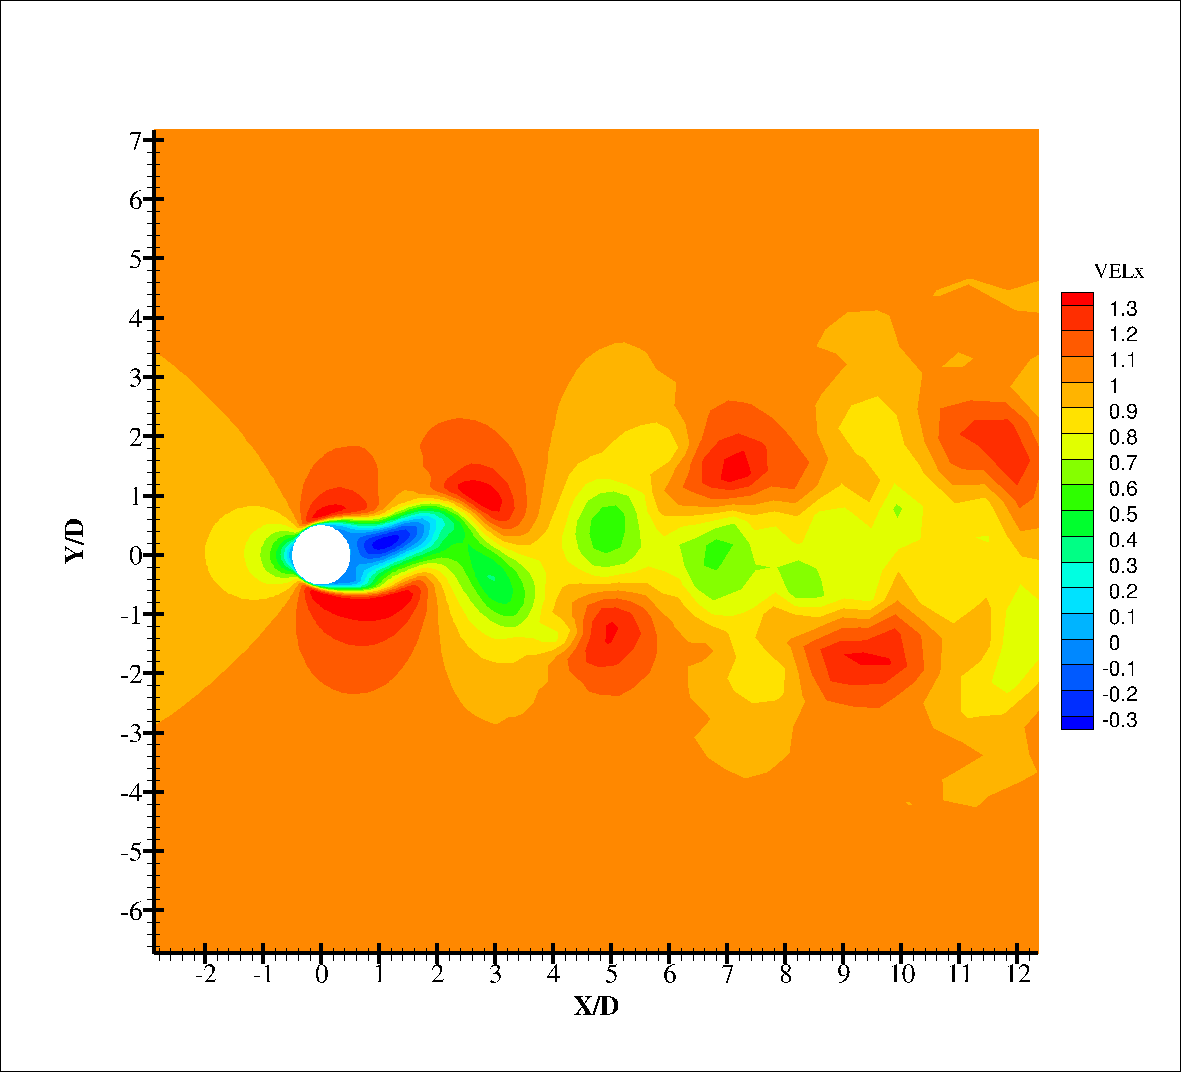
\includegraphics[height=2.6in]{Vx_182s}
%		\caption{t=182s}
%	\end{minipage}
%	
%	\begin{minipage}[t]{4cm}
%		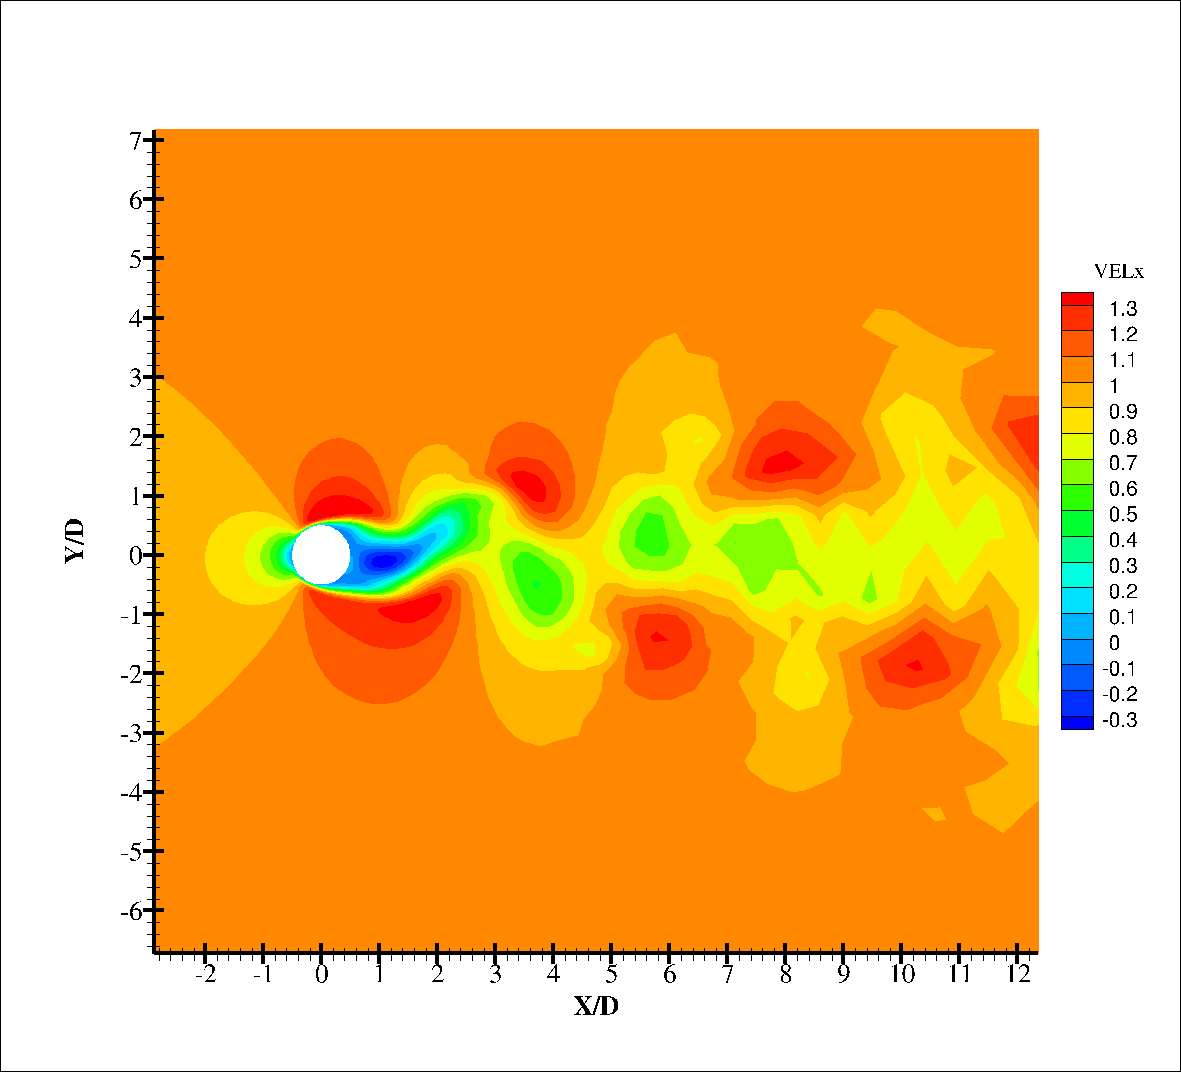
\includegraphics[height=2.6in]{Vx_183s}
%		\caption{t=183s}
%	\end{minipage}
%	\hspace{4cm}
%	\begin{minipage}[t]{4cm}
%%		\centering
%		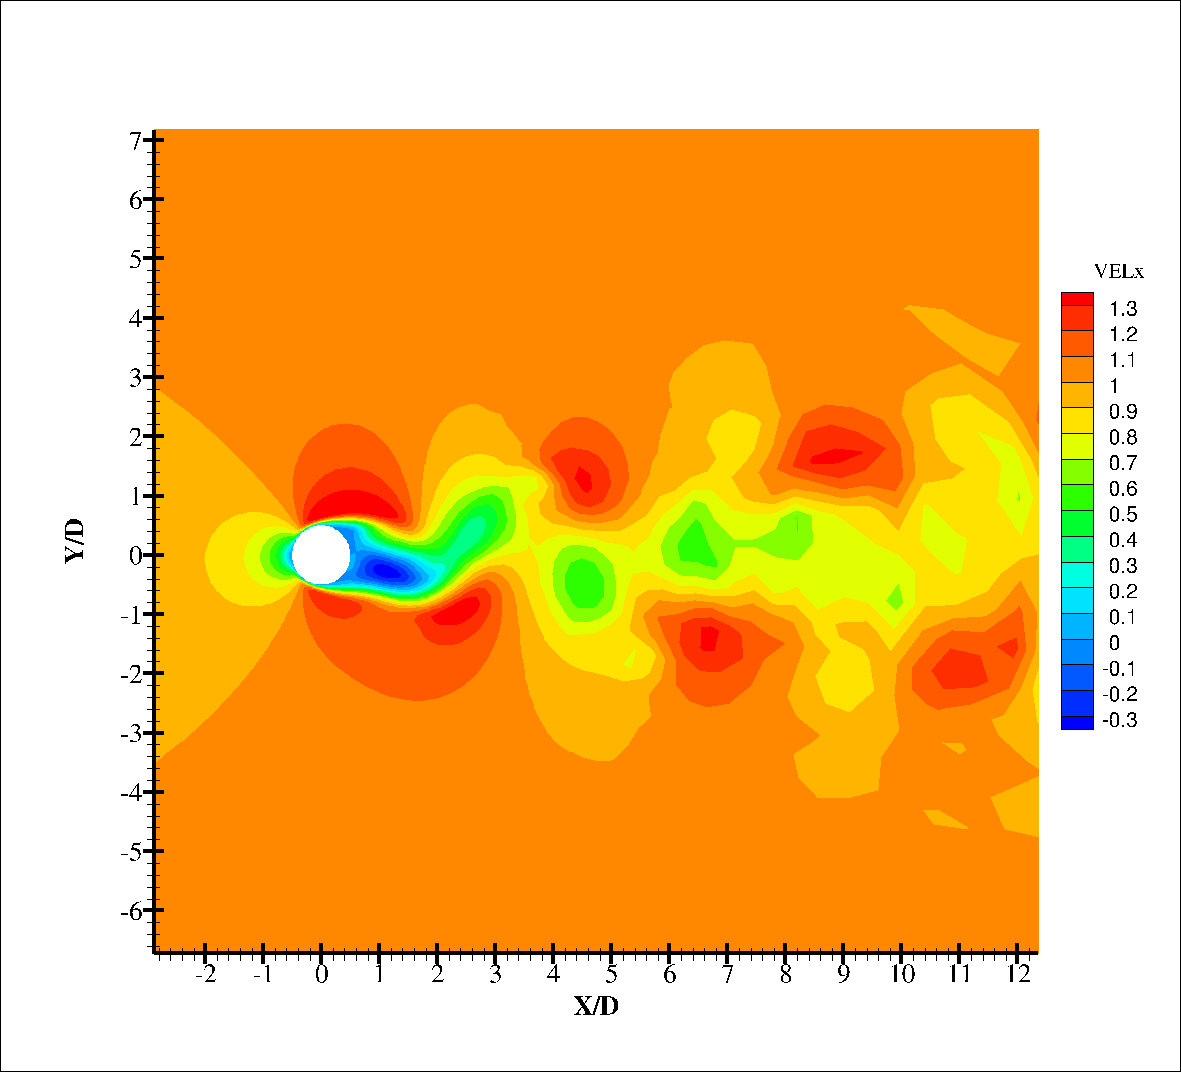
\includegraphics[height=2.6in]{Vx_184s}
%		\caption{t=184s}
%	\end{minipage}
%	
%	\begin{minipage}[t]{4cm}
%		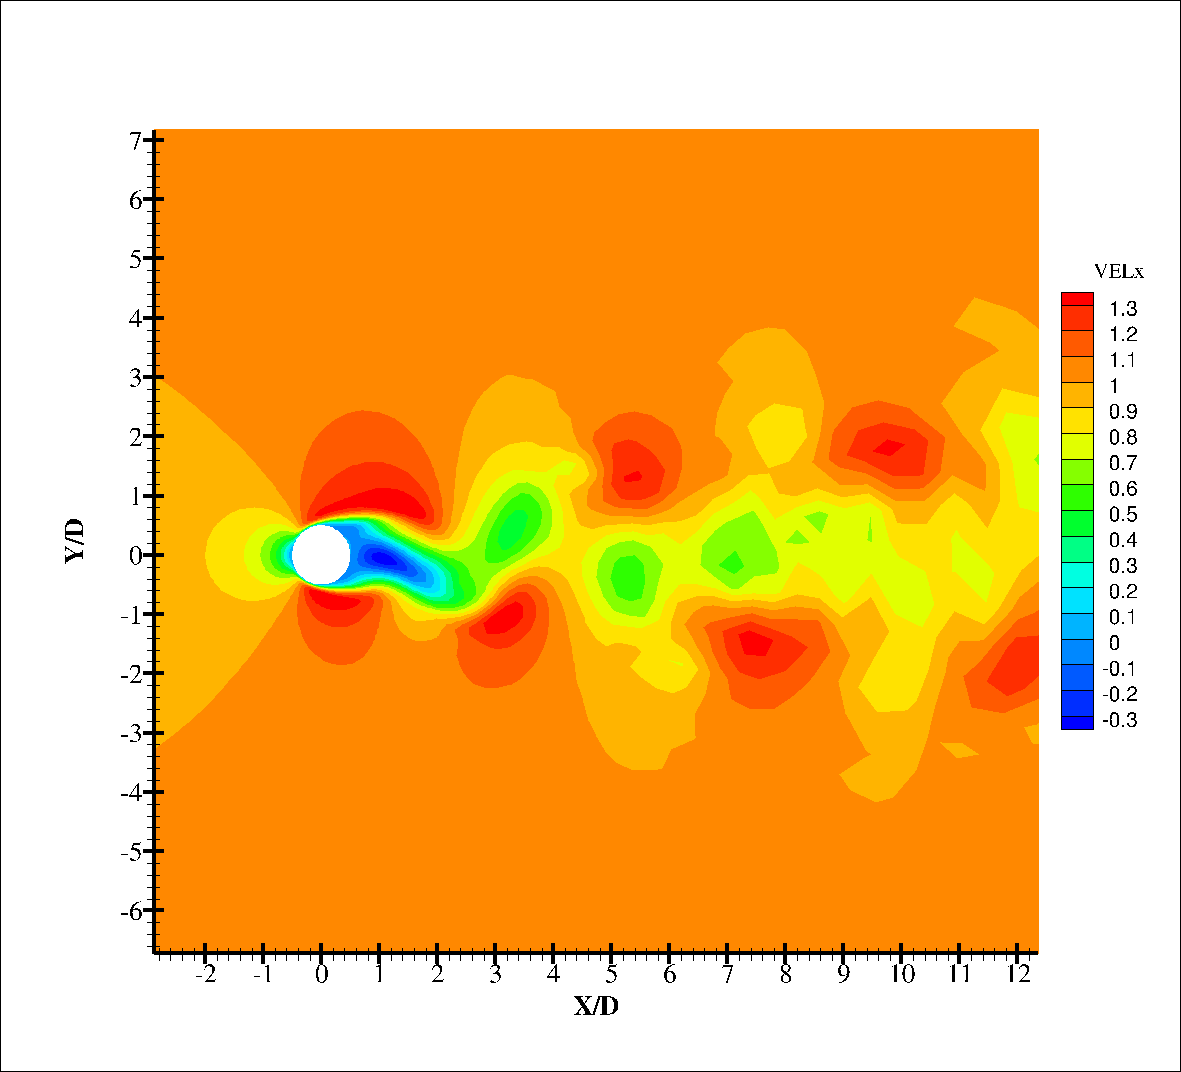
\includegraphics[height=2.6in]{Vx_185s}
%		\caption{t=185s}
%	\end{minipage}
%	\hspace{4cm}
%	\begin{minipage}[t]{4cm}
%%		\centering
%		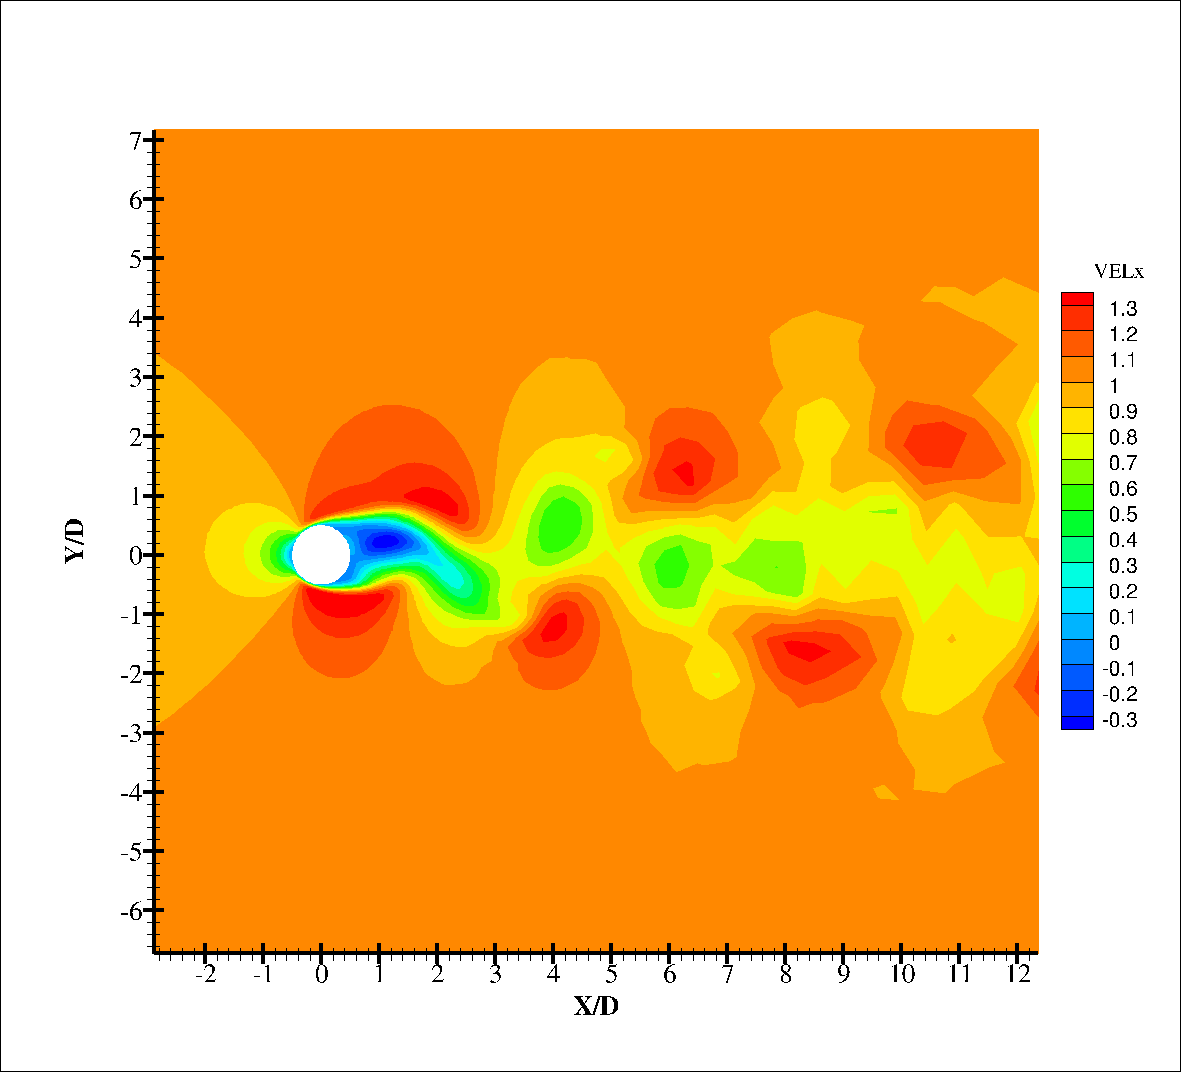
\includegraphics[height=2.6in]{Vx_186s}
%		\capt[ion{t=186s}
%	\end{minipage}
%\caption{Instantaneous velocity contour}
%\label{fig:4.2}
%\end{figure}

\begin{figure}[H]
\centering
	\begin{subfigure}[t]{7cm}
		\fbox{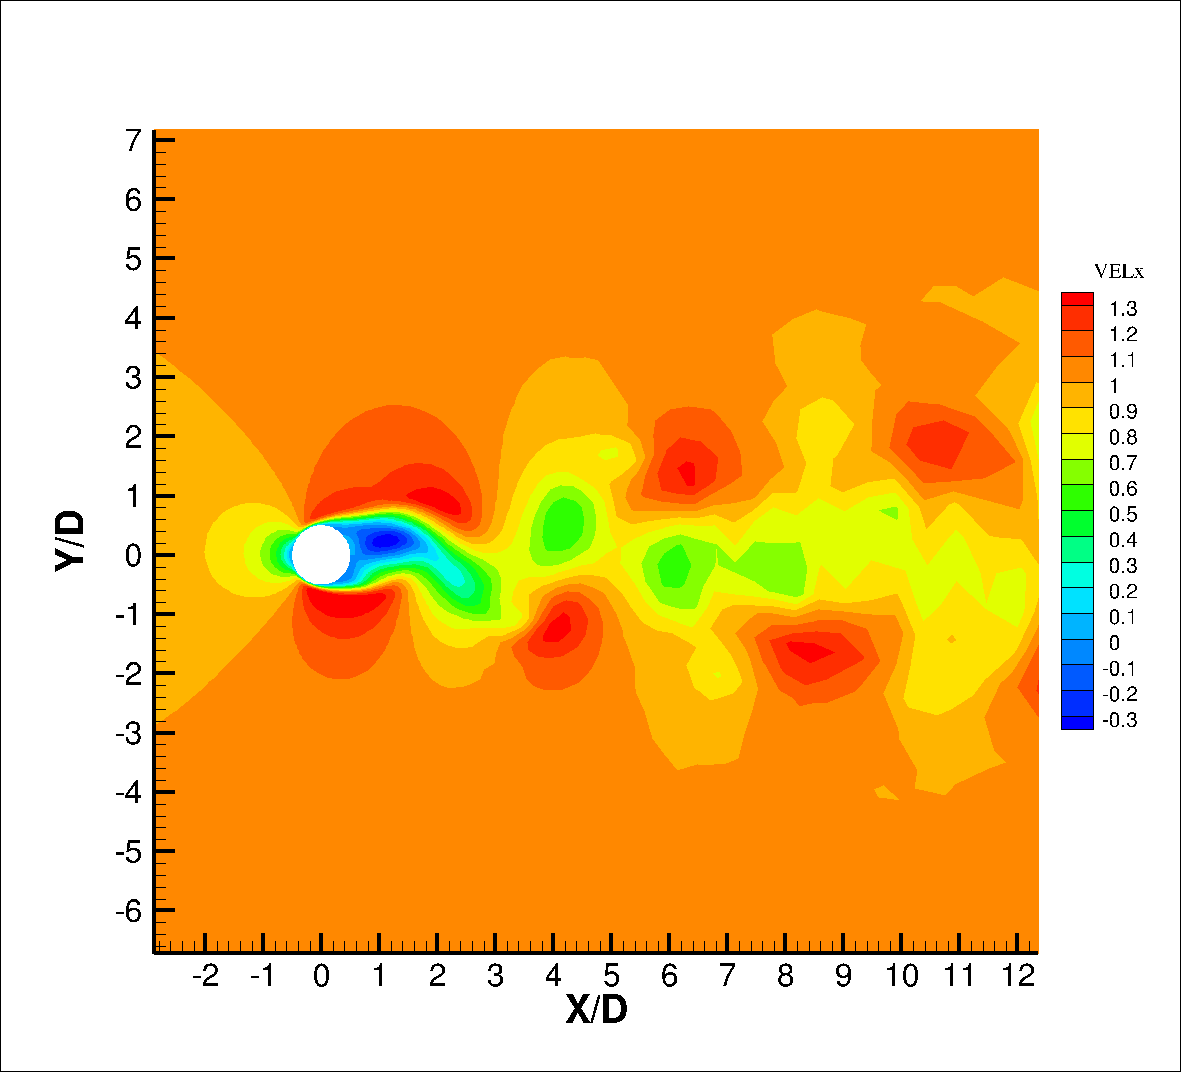
\includegraphics[width=6.5cm]{Vx_181s}}
		\caption{t=181s}
	\end{subfigure}
%	\hspace{4cm}
	\begin{subfigure}[t]{7cm}
%		\centering
		\fbox{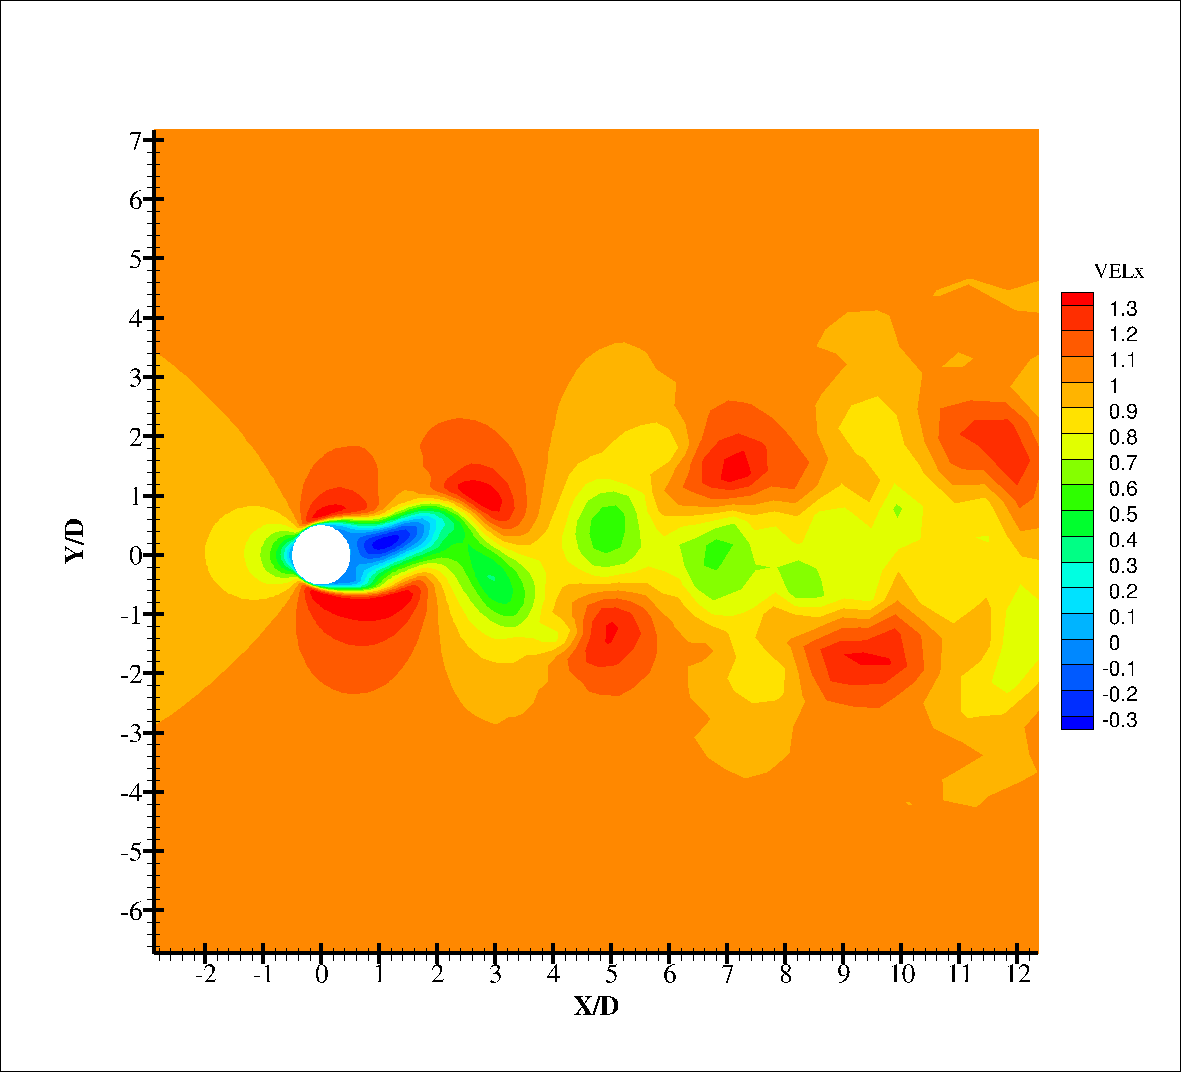
\includegraphics[width=6.5cm]{Vx_182s}}
		\caption{t=182s}
	\end{subfigure}
	
	\begin{subfigure}[t]{7cm}
		\fbox{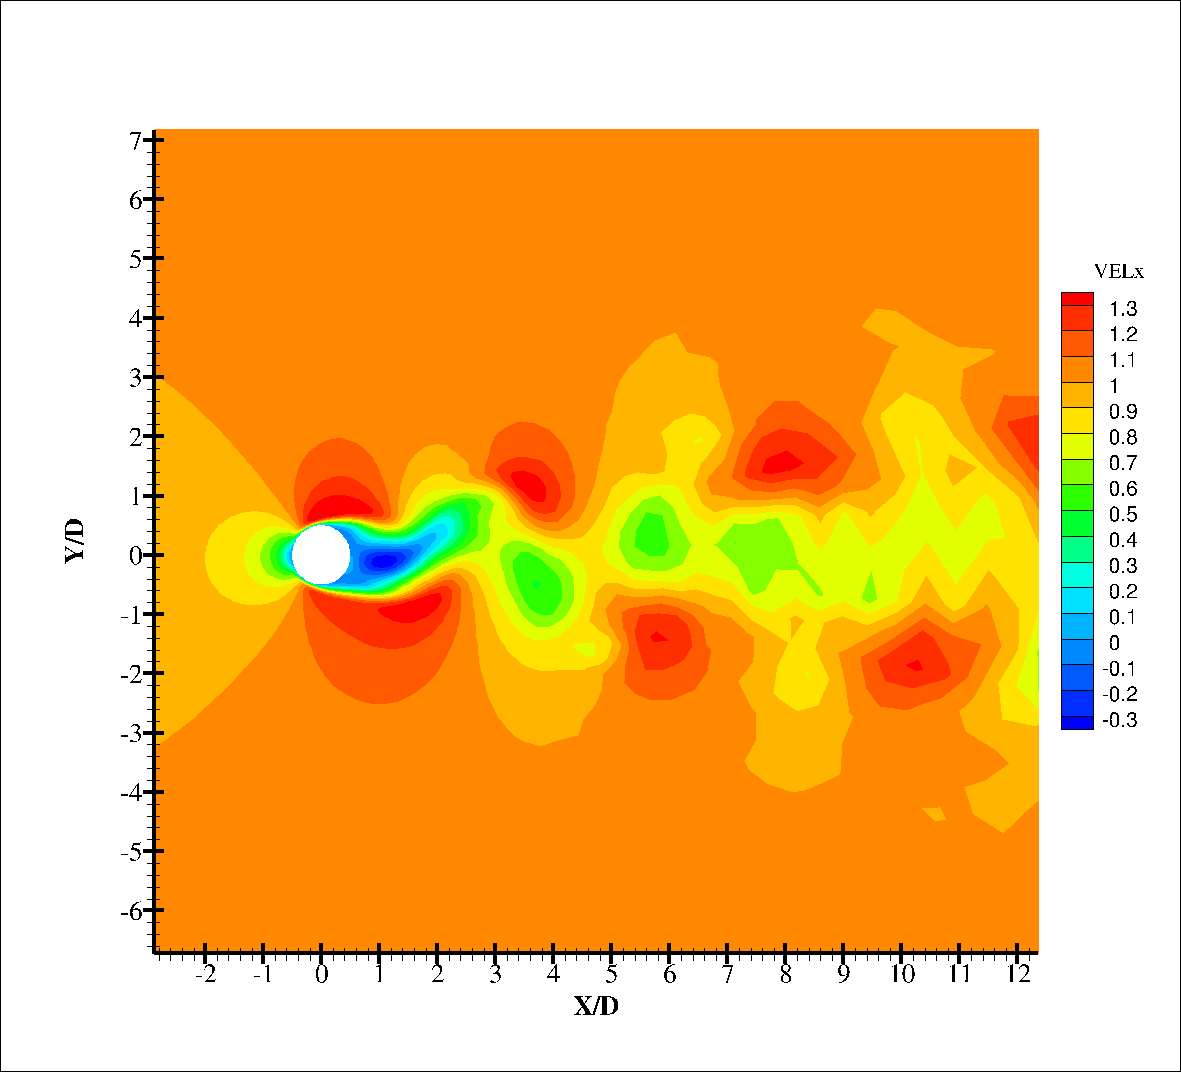
\includegraphics[width=6.5cm]{Vx_183s}}
		\caption{t=183s}
	\end{subfigure}
%	\hspace{4cm}
	\begin{subfigure}[t]{7cm}
%		\centering
		\fbox{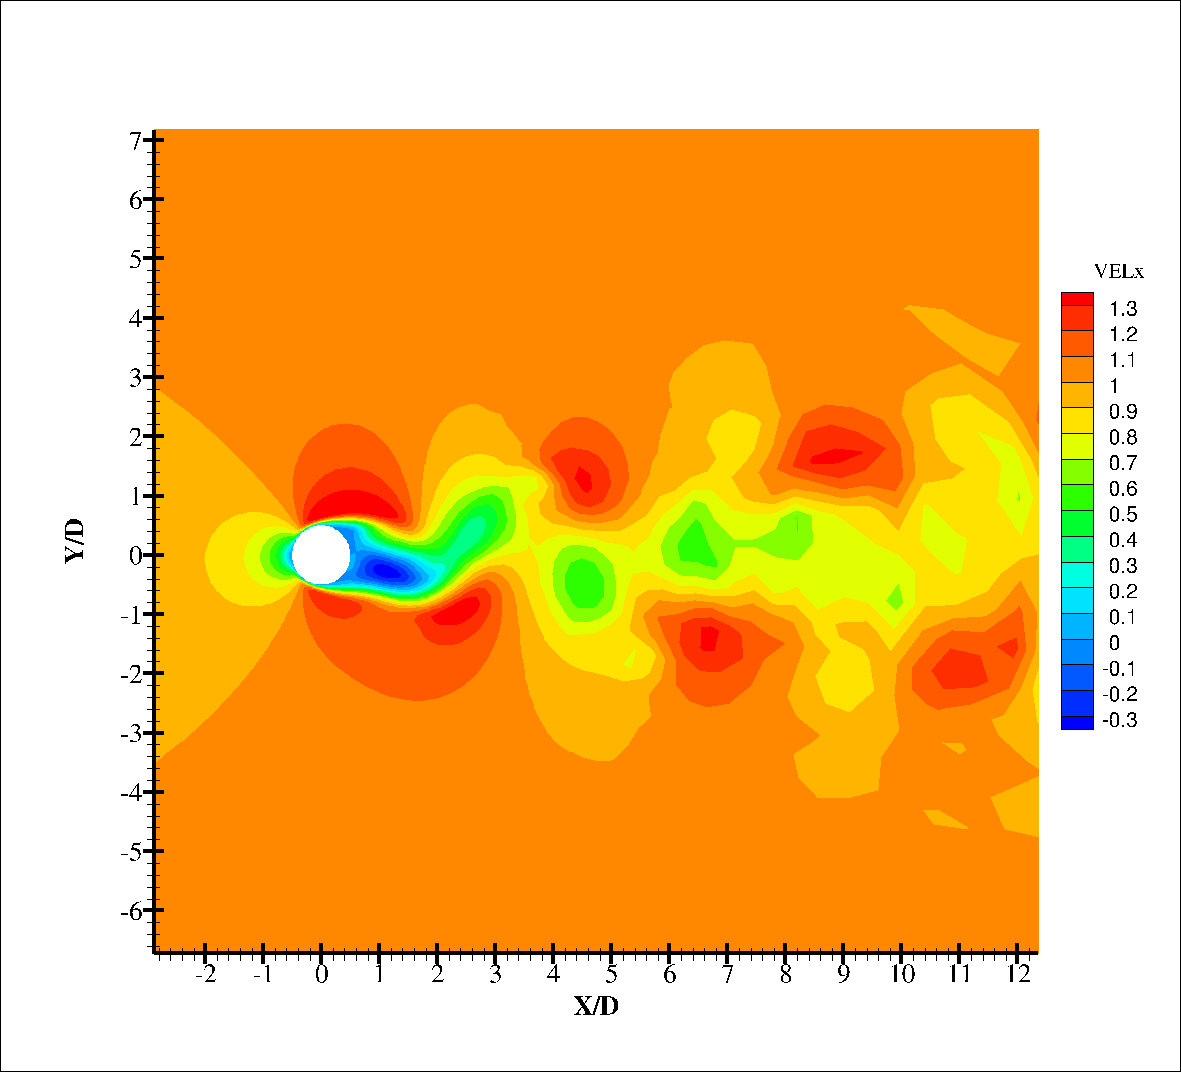
\includegraphics[width=6.5cm]{Vx_184s}}
		\caption{t=184s}
	\end{subfigure}
	
	\begin{subfigure}[t]{7cm}
		\fbox{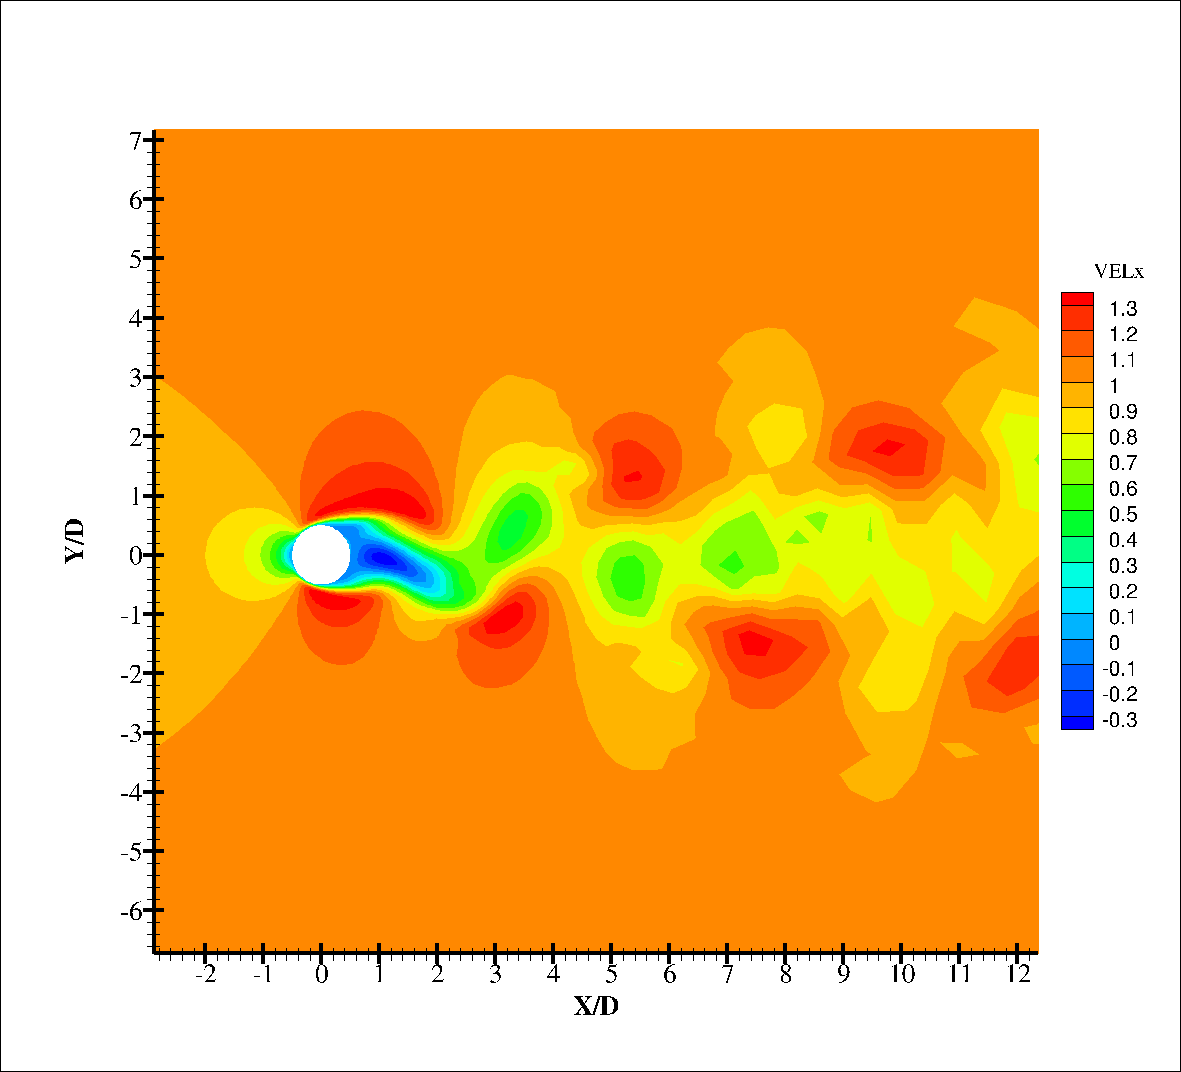
\includegraphics[width=6.5cm]{Vx_185s}}
		\caption{t=185s}
	\end{subfigure}
%	\hspace{4cm}
	\begin{subfigure}[t]{7cm}
%		\centering
		\fbox{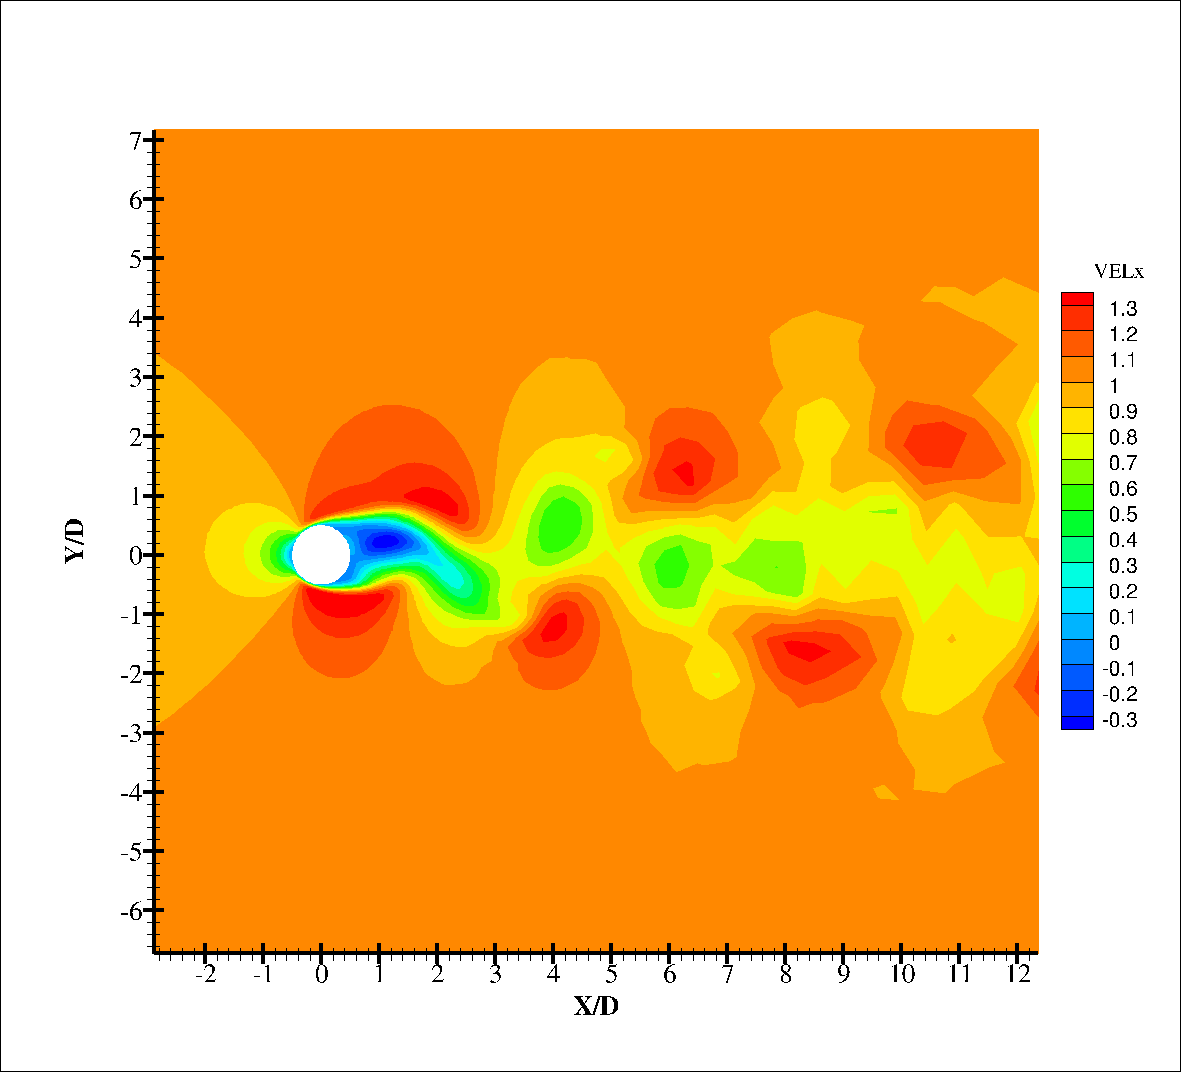
\includegraphics[width=6.5cm]{Vx_186s}}
		\caption{t=186s}
	\end{subfigure}
\caption{Instantaneous velocity contour}
\label{fig:4.2}
\end{figure}

\begin{figure}[H]
\centering
	\begin{subfigure}[t]{7cm}
		\fbox{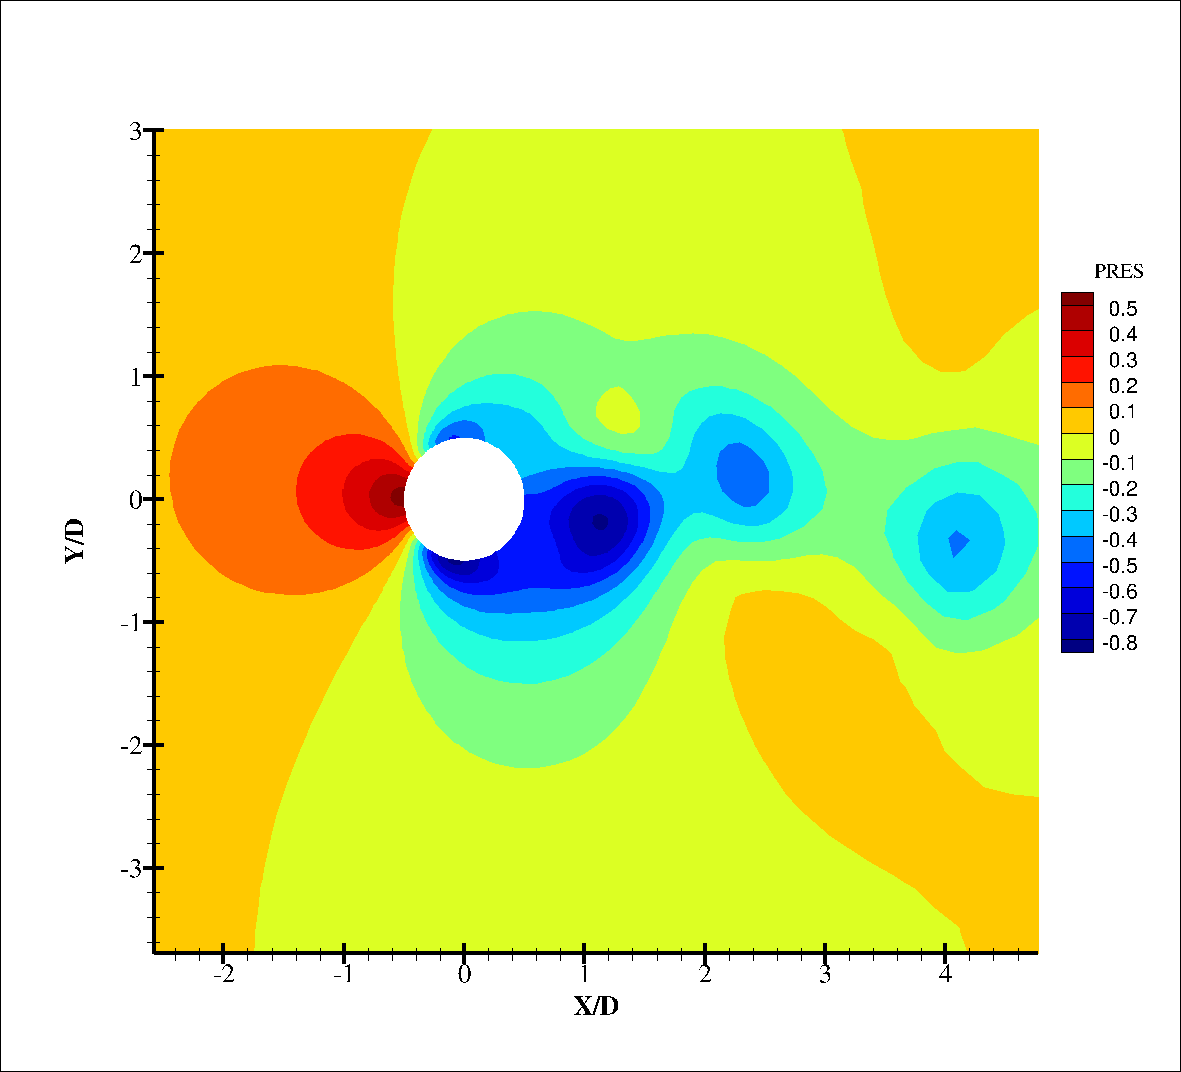
\includegraphics[width=6.5cm]{Pr_cyl_181s}}
		\caption{t=181s}
	\end{subfigure}
%	\hspace{4cm}
	\begin{subfigure}[t]{7cm}
%		\centering
		\fbox{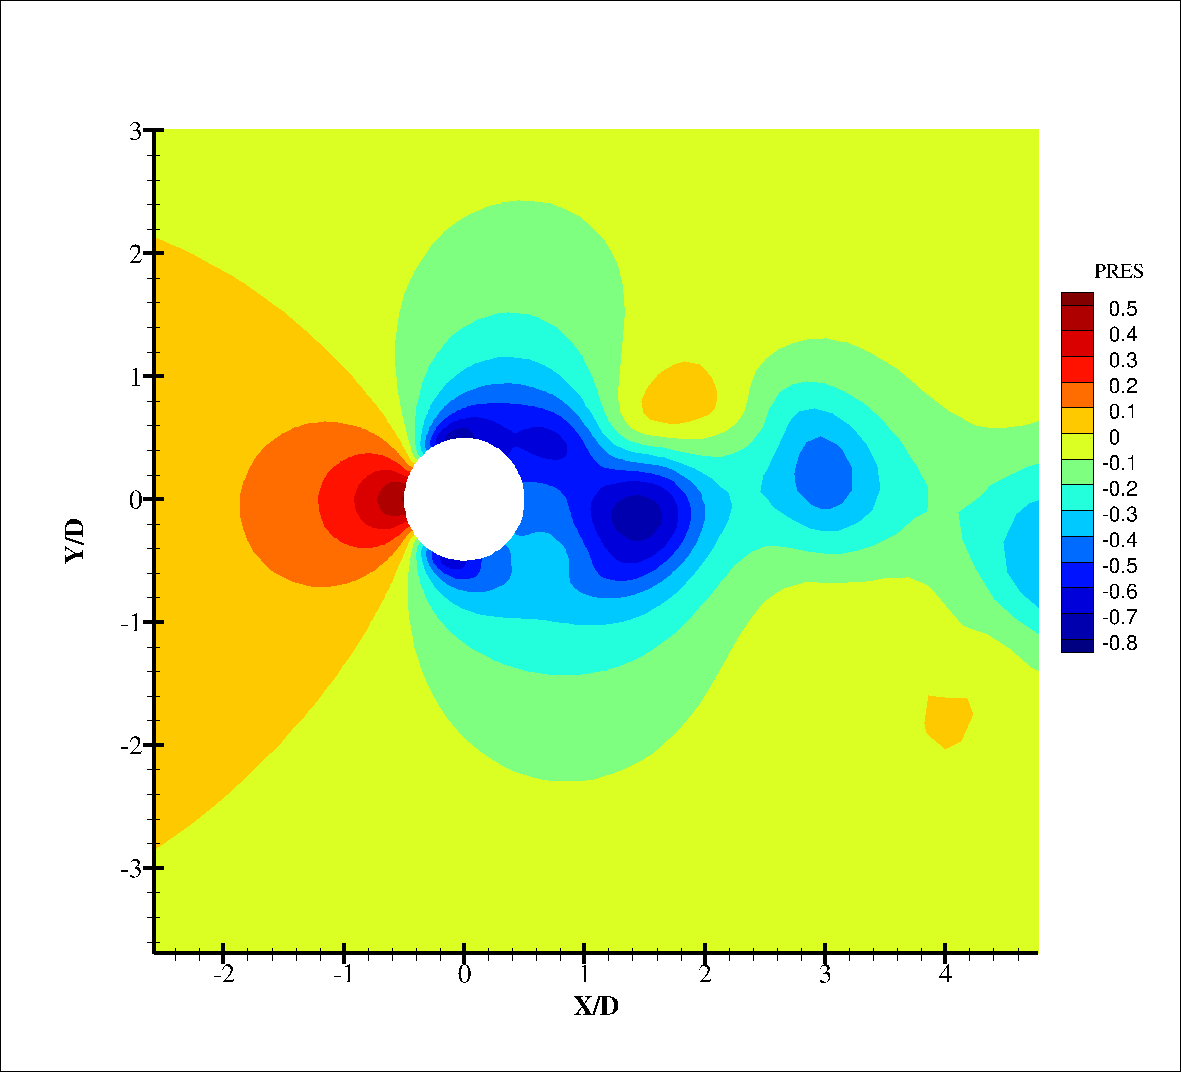
\includegraphics[width=6.5cm]{Pr_cyl_182s}}
		\caption{t=182s}
	\end{subfigure}
	
	\begin{subfigure}[t]{7cm}
		\fbox{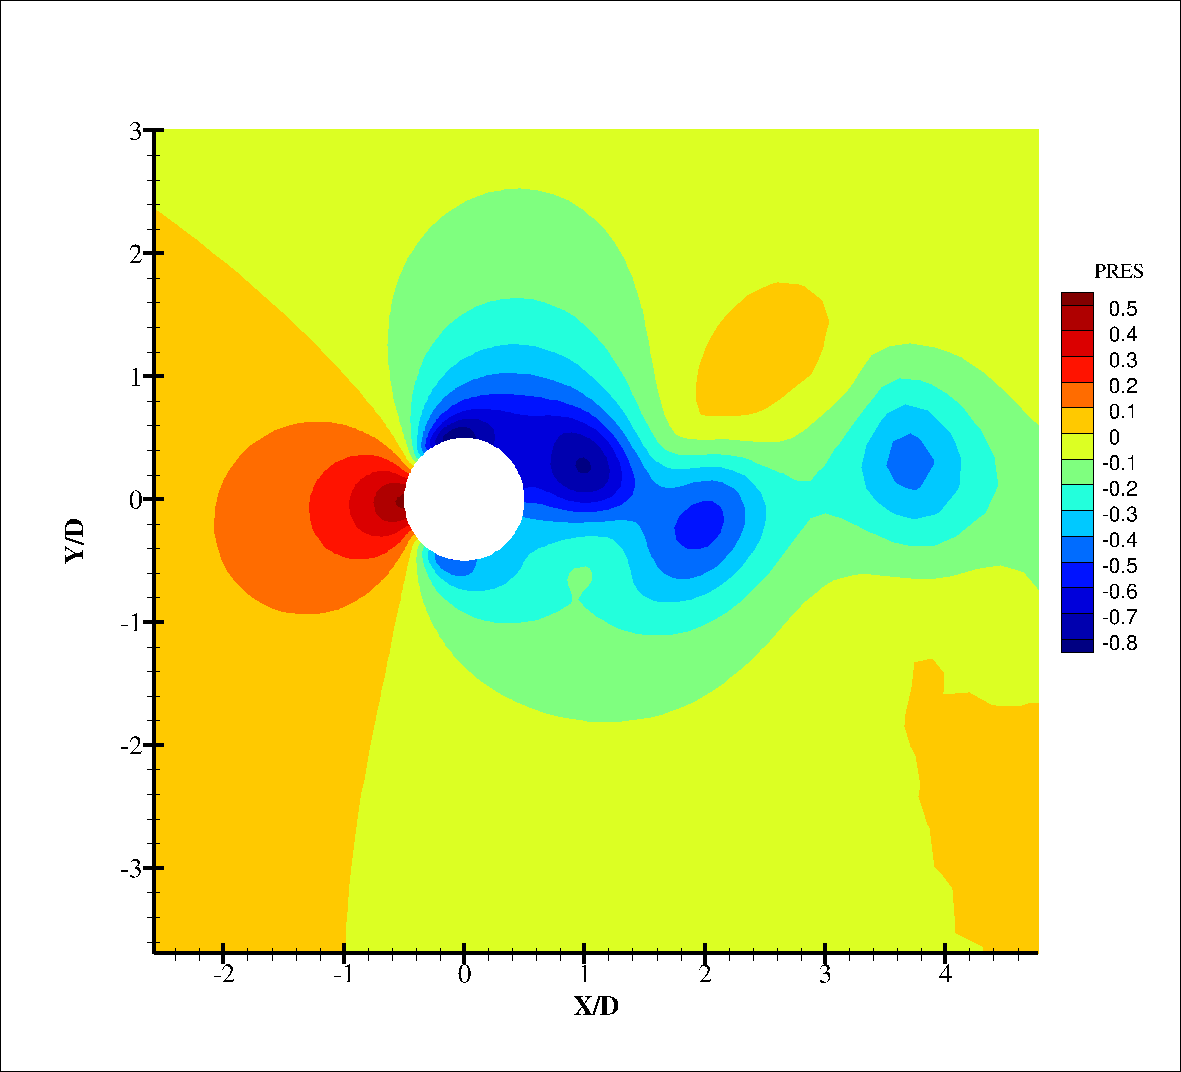
\includegraphics[width=6.5cm]{Pr_cyl_183s}}
		\caption{t=183s}
	\end{subfigure}
%	\hspace{4cm}
	\begin{subfigure}[t]{7cm}
%		\centering
		\fbox{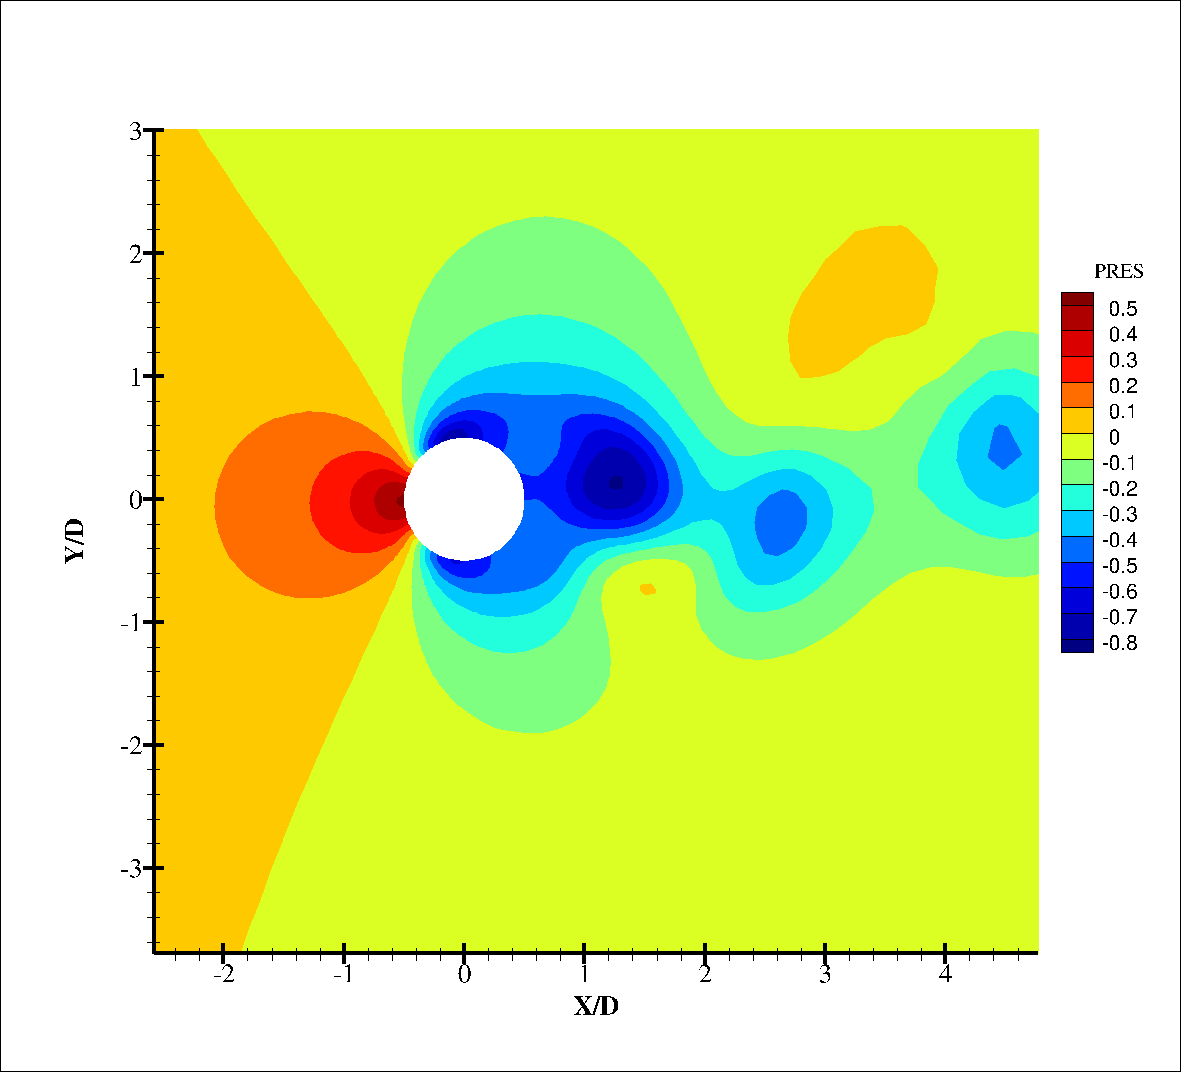
\includegraphics[width=6.5cm]{Pr_cyl_184s}}
		\caption{t=184s}
	\end{subfigure}
	
	\begin{subfigure}[t]{7cm}
		\fbox{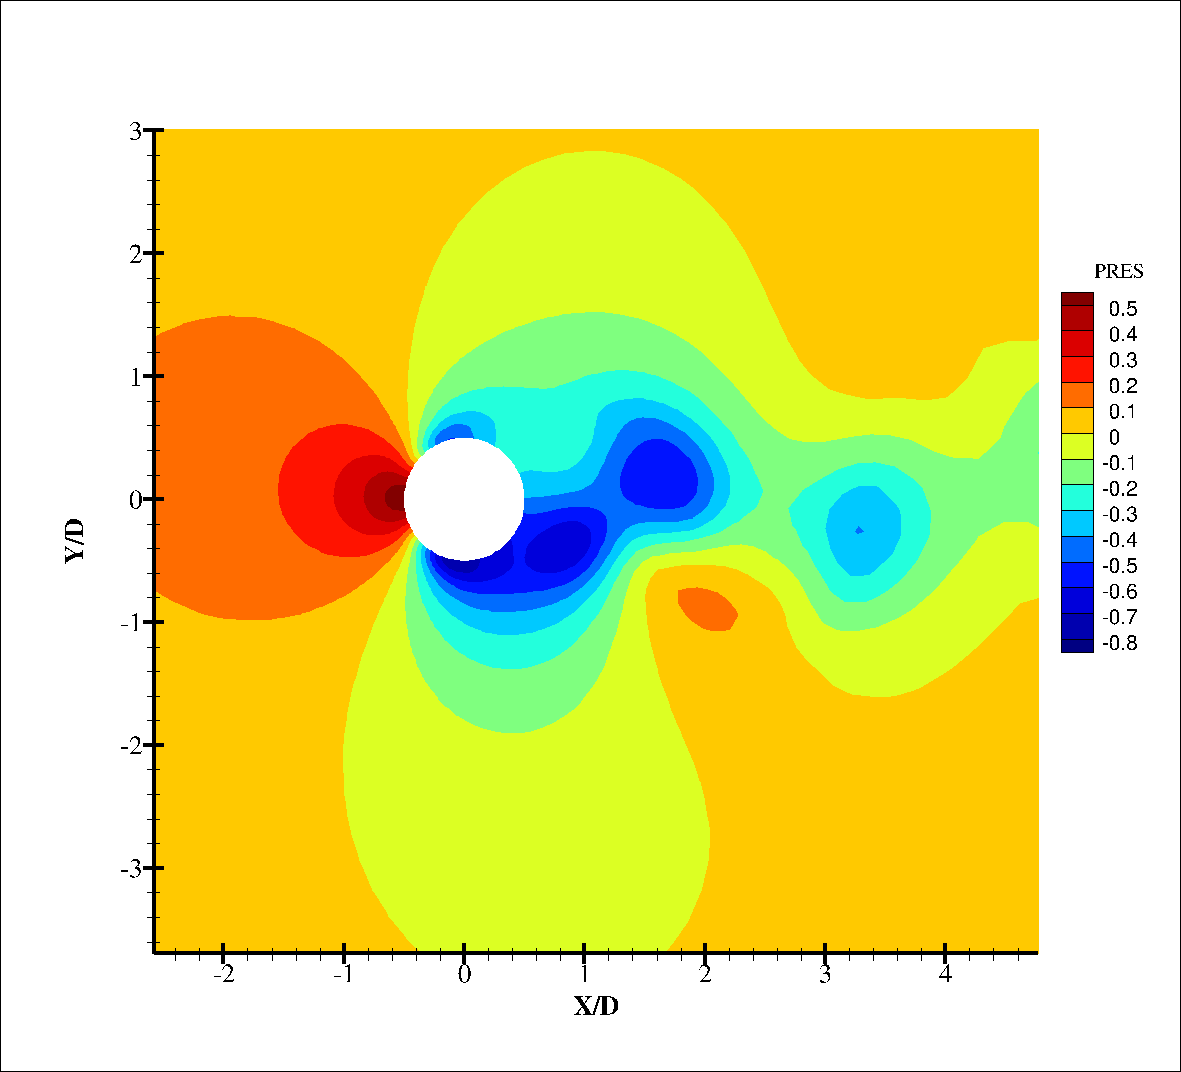
\includegraphics[width=6.5cm]{Pr_cyl_185s}}
		\caption{t=185s}
	\end{subfigure}
%	\hspace{4cm}
	\begin{subfigure}[t]{7cm}
%		\centering
		\fbox{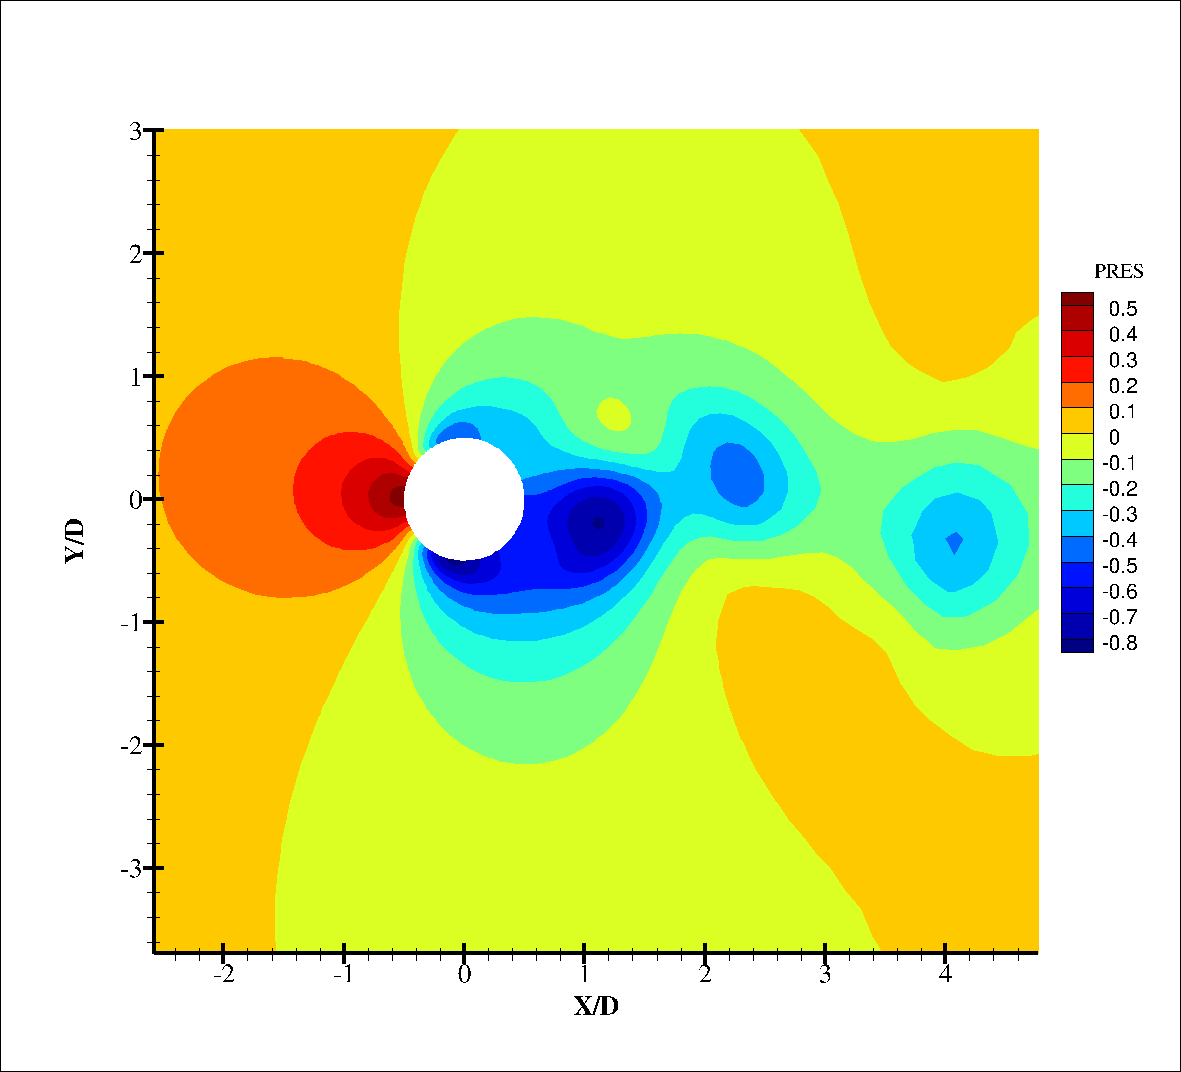
\includegraphics[width=6.5cm]{Pr_cyl_186s}}
		\caption{t=186s}
	\end{subfigure}
\caption{Instantaneous pressure contour}
\label{fig:4.3}
\end{figure}

The \textit{lift} $C_l$ and \textit{drag} $C_d$ coefficients are calculated using the following formulae:

\begin{align}
C_d &= \frac{F_x}{\frac{1}{2} \rho A U_{\infty}^{2}}\\
C_l &= \frac{F_y}{\frac{1}{2} \rho A U_{\infty}^{2}}
\end{align}

In the figure \ref{fig:4.4} the variation of lift and drag coefficients over time is presented. It can be observed that the lift force settles to a sinusoidal pattern after the wake of instability leads to vortex shedding. The root mean square (rms) value of lift coefficient is calculated to be $C_{l_{rms}} = 0.3249$. Similarly, the drag force also follows a periodic behavior with the mean value calculated to be $\bar{C_d} = 1.1632$. 

\begin{figure}[H]
\centering
\fbox{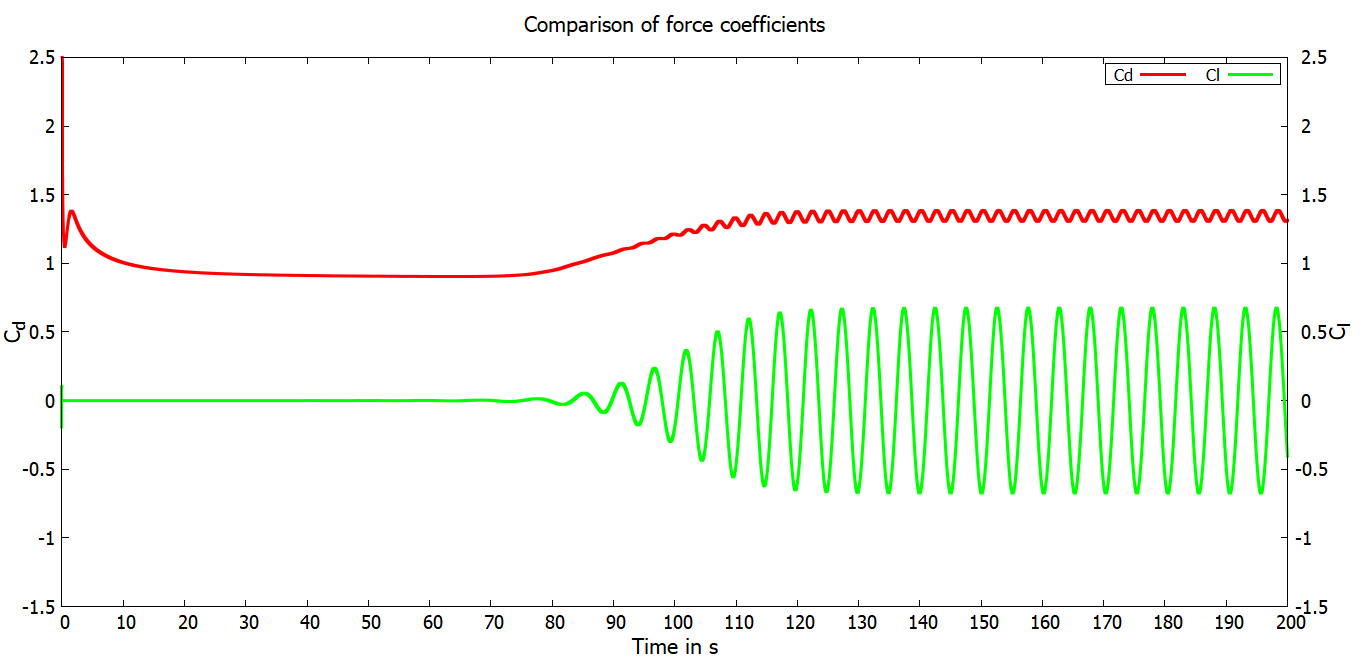
\includegraphics[width=\linewidth]{FC_flow_alone}}
\caption{Variation of Lift and Drag coefficients}
\label{fig:4.4}
\end{figure}

The Strouhal number (St) is a dimensionless number which describes the mechanisms of an oscillating flow. It is defined as,

\begin{equation}
St = \frac{f_s D}{U_\infty}
\end{equation}

where $f_s$ is the vortex shedding frequency. The strouhal number for lift and drag coefficients are calculated to be 0.1945 and 0.3839 respectively. The frequency of oscillation of the drag force is observed to be almost twice as that of lift force. These values are in good agreement to the values observed by \citet{zhou1999vortex}. The observed values are tabulated in \ref{table:4.3}.

\begin{table} [H]
\centering
	\begin{tabular}{|c|c|c|}
	\hline 
	\multirow{2}{*}{Values} & \multicolumn{2}{c|}{Force coefficients}\tabularnewline
	\cline{2-3} 
	 & Coefficient of drag ($C_{d}$) & Coefficient of lift ($C_{l}$)\tabularnewline
	\hline 
	Mean & 1.1632 & -\tabularnewline
	\hline 
	RMS & - & 0.3249\tabularnewline
	\hline 
	Strouhal number (St) & 0.3839 & 0.1945\tabularnewline
	\hline 
	Strouhal number Zhou et.al. (St) & 0.3853 & 0.1922\tabularnewline
	\hline 
	\end{tabular}
\caption{Characteristic values of lift and drag forces}
\label{table:4.3}
\end{table}

This simulation file is used as a restart file for some of the simulation cases of the Fluid-Structure Interaction problem.

\section{FSI simulation results}
The calculations were then performed for an elastic circular cylinder with two degrees of freedom for a number of cases. The values Re=200 and a Mass ratio M=1 is maintained constant through all simulation cases. The damping coefficient Sg is varied for values 1,0.1 and 0.01 respectively and its characteristics are studied. The simulations are carried out for FASTEST-3D with

\begin{enumerate}[(i)]
\item Constant URF (Constant)
\item Aitken URF method (Aitken)
\item Steepest Descent URF method (SD)
\end{enumerate}

The nomenclature given in the brackets for each method is followed in the plots, so as to provide brevity. These cases are simulated with and without a flow restart file, in which the flow field is established. The simulated cases are summarized in the table \ref{table:4.4}.

% Table generated by Excel2LaTeX from sheet 'Sheet1'
\begin{table}[htbp]
  \centering
  \setlength\aboverulesep{0pt}
  \setlength\belowrulesep{0pt} % to avoid discontinuous vertical lines
 \setcellgapes{3pt}\makegapedcells
   \scalebox{0.75}{
    \begin{tabular}{|c|l|c|c|c|c|c|c|}
    \toprule
          & \multicolumn{7}{c|}{M=1} \\
\cmidrule{2-8}          &       & \multicolumn{2}{c|}{Sg=1} & \multicolumn{2}{c|}{Sg=0.1} & \multicolumn{2}{c|}{Sg=0.01} \\
\cmidrule{3-8}          &       & \multicolumn{1}{l|}{With restart} & \multicolumn{1}{l|}{Without restart} & \multicolumn{1}{l|}{With restart} & \multicolumn{1}{l|}{Without restart} & \multicolumn{1}{l|}{With restart} & \multicolumn{1}{l|}{Without restart} \\
    \midrule
    \multirow{3}[6]{*}{FASTEST 3-D with} & Constant URF & x     & x     & x     & x     & x     & x \\
\cmidrule{2-8}          & Aitken URF & x     & x     & x     & x     & x     & x \\
\cmidrule{2-8}          & SD URF & x     & x     & x     & x     & x     & x \\
    \bottomrule
    \end{tabular}%%
   }
  \caption{Summary of the various cases simulated}
  \label{table:4.4}%
\end{table}%

The following nomenclature has been followed henceforth for identifying the different simulation cases:

\begin{enumerate}[(a)]
\item case 1 : Mass ratio M=1 and damping coefficient Sg=1
\item case 2 : Mass ratio M=1 and damping coefficient Sg=0.1
\item case 3 : Mass ratio M=1 and damping coefficient Sg=0.01
\end{enumerate}

\subsection{Determining a suitable constant value of URF}
The simulations were performed considering 50 sub-iterations as the upper limit for convergence of the FSI solver within a time step. To determine a suitable constant value for under-relaxation factor (URF) simulations were carried out for all the cases with different URF values. The simulations were performed on 8 cores for a total of 10,000 time steps. The average sub-iterations taken per time step for various cases is summarized in the table \ref{table:4.5}.\\

\begin{table}[htbp]
  \centering
  	\begin{tabular}{|c|c|c|c|}
	\hline 
	\multirow{2}{*}{FASTEST-3D with constant URF values} & \multicolumn{3}{c|}{Average sub-iterations per timestep}\tabularnewline
	\cline{2-4} 
	 & case 1 & case 2  & case 3\tabularnewline
	\hline 
	0.2 & 32 & 36 & 31\tabularnewline
	\hline 
	0.4 & 14 & 17 & 14\tabularnewline
	\hline 
	0.6 & 15 & 15 & 14\tabularnewline
	\hline 
	\rowcolor[rgb]{ .573,  .816,  .314} 0.8 & 13 & 13 & 11\tabularnewline
	\hline 
	1 & 16 & 16 & 12\tabularnewline
	\hline 
	\end{tabular}
  \caption{Average number of sub iterations per time step}
  \label{table:4.5}%
\end{table}%

The constant URF value of 0.8 gave an average sub-iteration count of around 13 for each of the simulated cases. This value is observed to be an optimum value and the same value has been considered for further simulations.

\subsection{Results for case 1: M=1 and Sg=1}
This section deals with the presentation and discussion of results for the case simulated with Mass ratio M=1 and damping coefficient Sg=1. Each simulation is performed for a total of around 50 vortex shedding cycles and with a frequency ratio $f_n/f_s = 1$. $f_n$ is the natural frequency of the cylinder.

The following nomenclature is followed to represent the characteristic behavior of the system.

\begin{enumerate}[(i)]
\item Mean value of drag coefficient ($\bar{C_d}$)
\item Root Mean Square (RMS) value of lift coefficient ($C_{l,rms}$)
\item Minimum displacement value along flow direction (${X/D}_{min}$)
\item Maximum displacement value along flow direction (${X/D}_{max}$)
\item Minimum displacement value perpendicular to the flow direction (${Y/D}_{min}$)
\item Maximum displacement value perpendicular to the flow direction (${Y/D}_{max}$)
\item Peak-to-peak vibration amplitude ($2 {Y_{rms}}/D$)
\end{enumerate}

All the values are non-dimensionalized in order to have a comparison with the work of \citet{zhou1999vortex}. 

\subsubsection{Without a restart file}
In this simulation, the cylinder is suspended from the initial time. The characteristics of the system is studied. Flow-induced vibrations are in general observed to be non-linear. The vibration of the structure affects the fluid flow around the structure which, in turn, changes the induced forces on the structure and thus the structural response. 

In the figure \ref{fig:4.6} the velocity pattern of the flow field is represented for a time period of 2.5s, which is approximately the time taken for one period of oscillation of the cylinder. From the velocity pattern, it can be observed that the flow pattern is affected in the near wake region of the cylinder. The difference can be observed when compared with the rigid cylinder case, where the vortex shedding was symmetrical. The vortex spacing between the opposing vortices is observed to be narrower in the streamwise direction and wider in the transverse direction. In the figure \ref{fig:4.7} the pressure attributed to these flow characteristics can be observed.

The following nomenclature for the simulation with different under relaxation factor schemes is :

\begin{enumerate}[(a)]
\item FASTEST-3D with constant URF value of 0.8: Constant
\item FASTEST-3D with Aitken URF scheme: Aitken
\item FASTEST-3D with Steepest Descent URF scheme: SD
\end{enumerate} 

In the figure \ref{fig:4.5} the variation of force coefficients $C_d$ and $C_l$ is plotted for a certain period of time steps. It can be observed that the onset of the oscillations are little different for each of the relaxation schemes. This is attributed to the varying number of sub-iterations for each scheme and hence, the convergence of the solver varies per time step. 

\begin{figure}[H]
\centering
\fbox{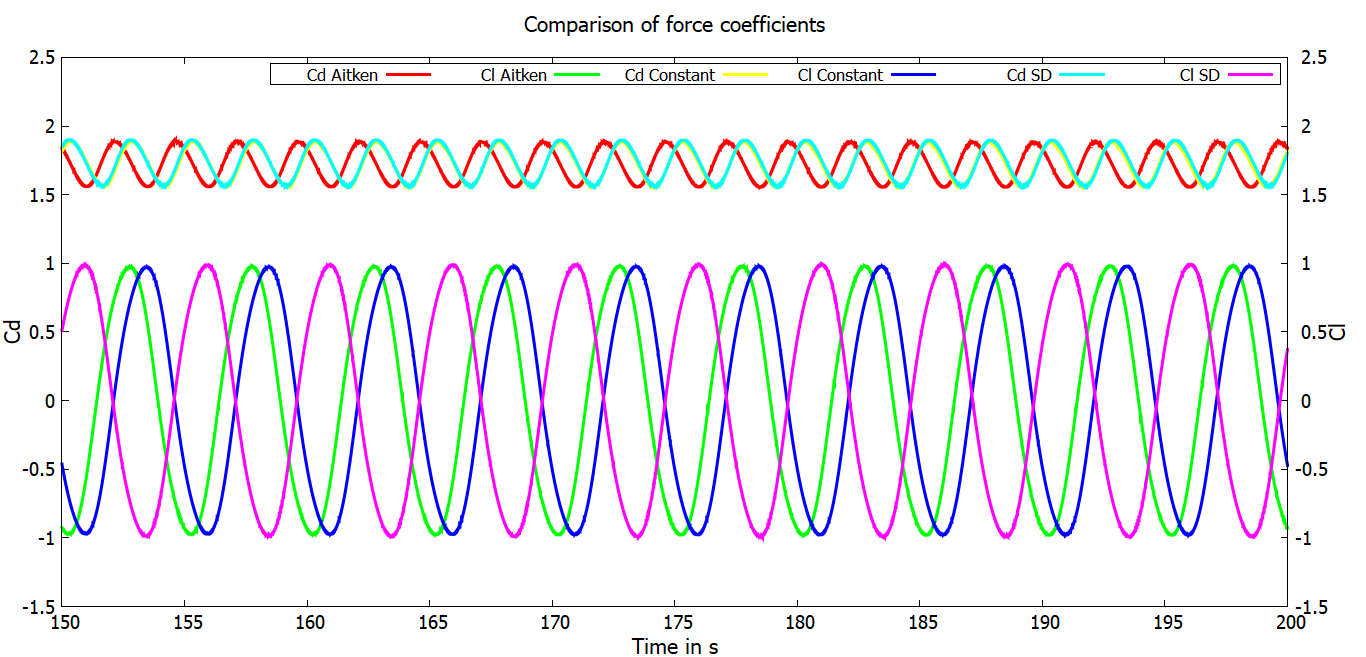
\includegraphics[width=\linewidth]{FC_Sg1_wor}}
\caption{Variation of Drag and Lift coefficients for case 1 without any restart}
\label{fig:4.5}
\end{figure}


\begin{figure}[H]
\centering
	\begin{subfigure}[t]{7cm}
		\fbox{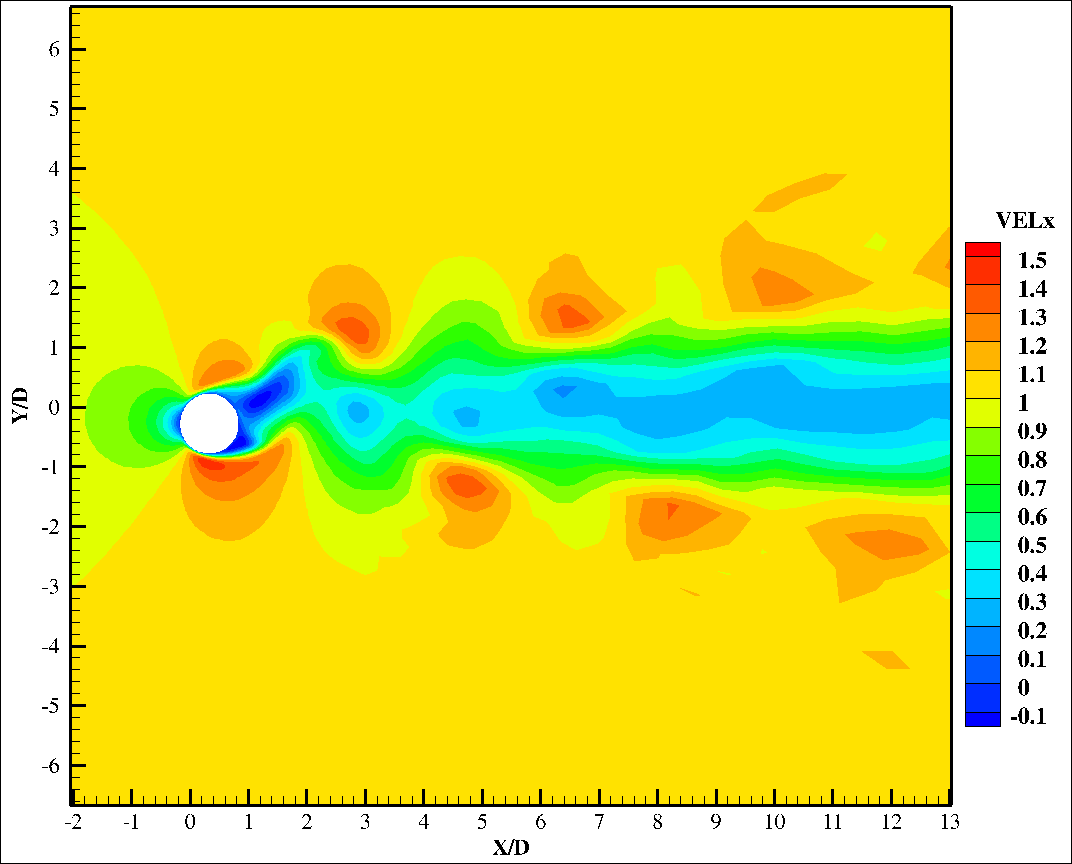
\includegraphics[width=6.5cm]{Sg_1_wor_Vel_150_5s}}
		\caption{t=150.5s}
	\end{subfigure}
%	\hspace{4cm}
	\begin{subfigure}[t]{7cm}
%		\centering
		\fbox{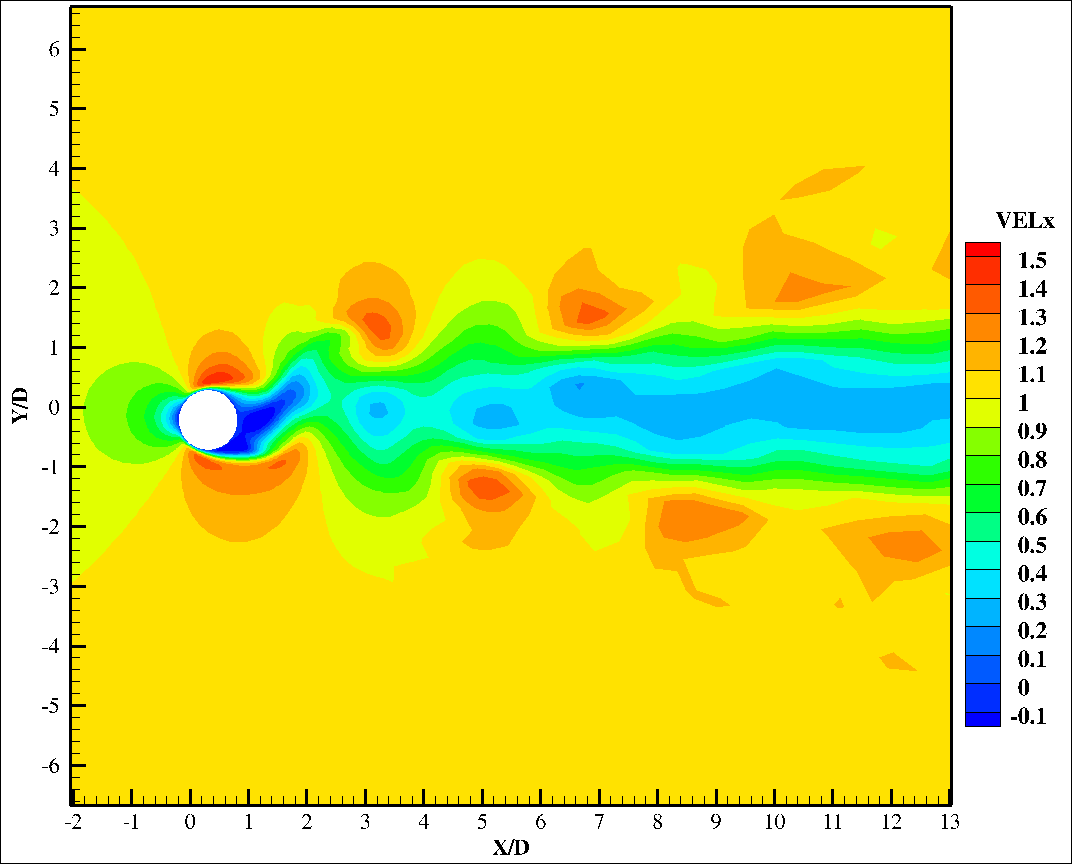
\includegraphics[width=6.5cm]{Sg_1_wor_Vel_151s}}
		\caption{t=151s}
	\end{subfigure}
	
	\begin{subfigure}[t]{7cm}
		\fbox{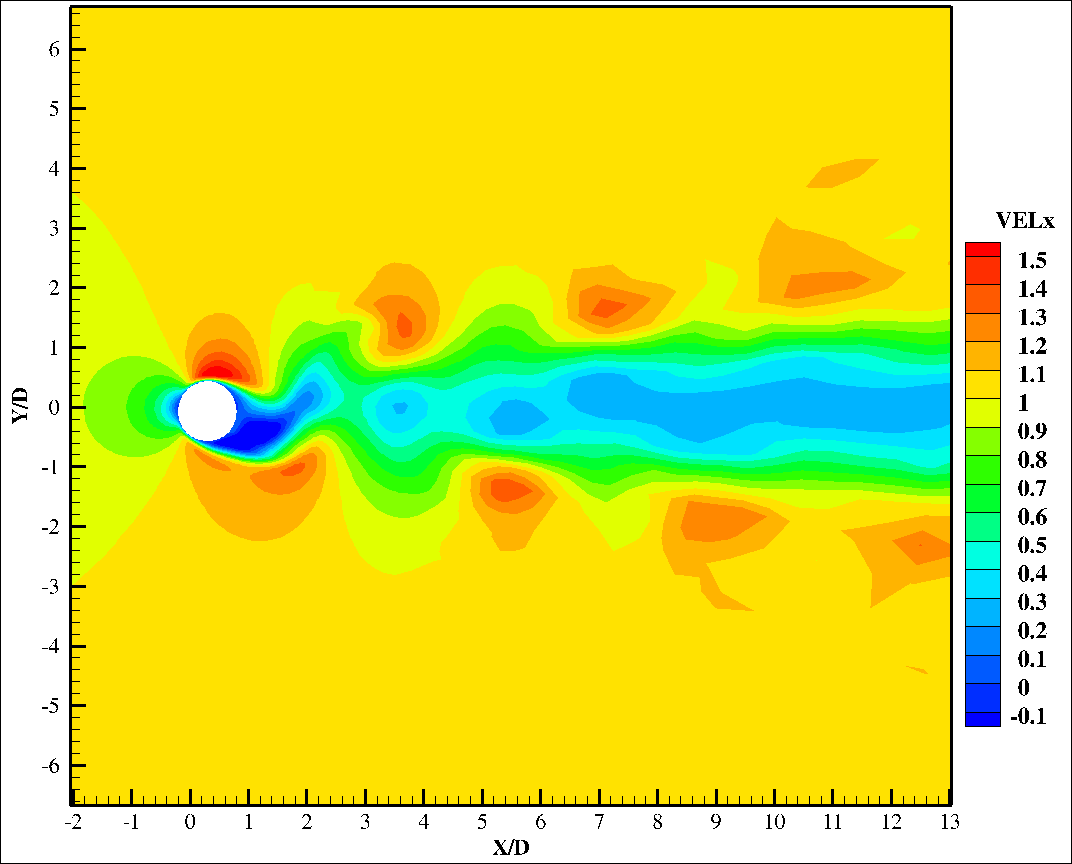
\includegraphics[width=6.5cm]{Sg_1_wor_Vel_151_5s}}
		\caption{t=151.5s}
	\end{subfigure}
%	\hspace{4cm}
	\begin{subfigure}[t]{7cm}
%		\centering
		\fbox{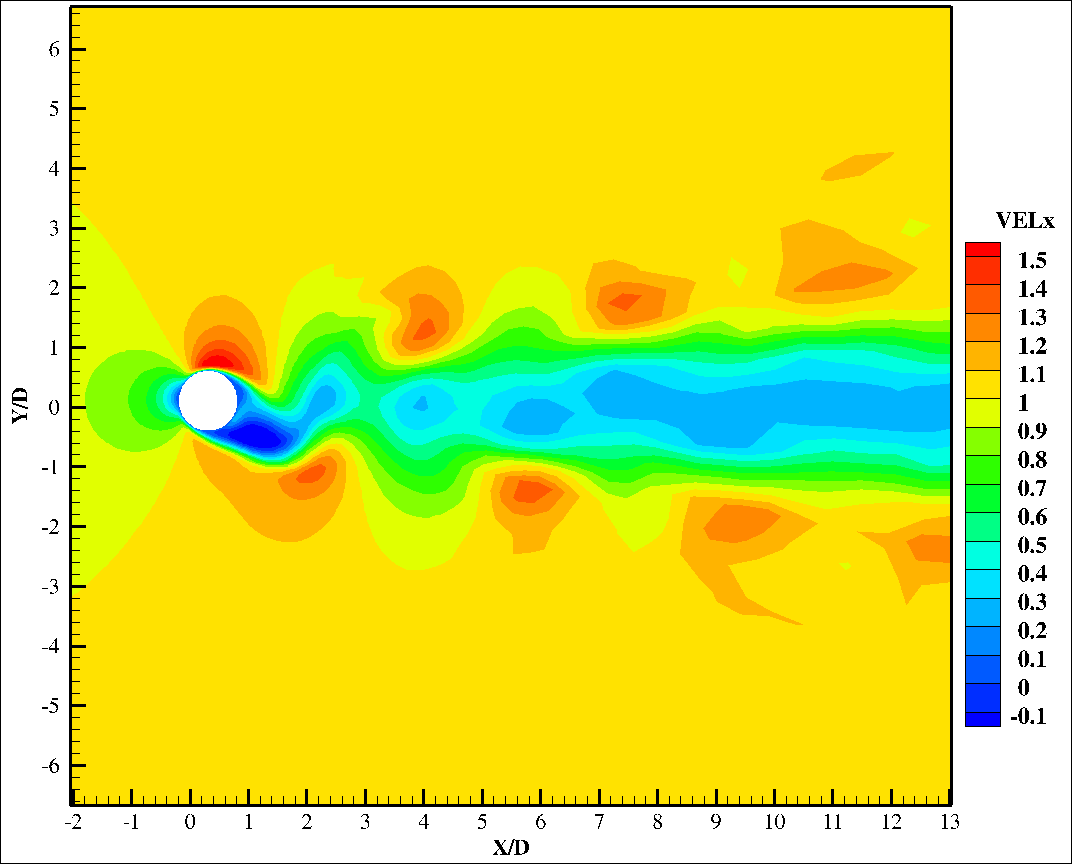
\includegraphics[width=6.5cm]{Sg_1_wor_Vel_152s}}
		\caption{t=152s}
	\end{subfigure}
	
	\begin{subfigure}[t]{7cm}
		\fbox{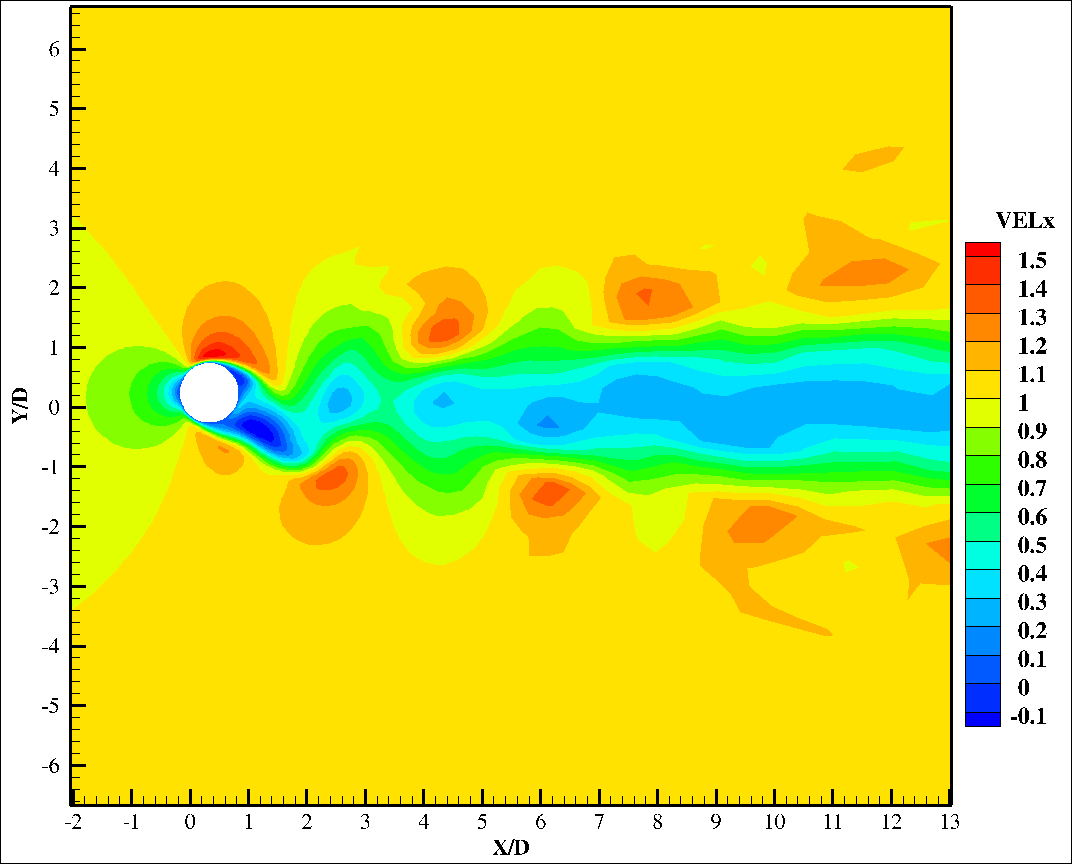
\includegraphics[width=6.5cm]{Sg_1_wor_Vel_152_5s}}
		\caption{t=152.5s}
	\end{subfigure}
%	\hspace{4cm}
	\begin{subfigure}[t]{7cm}
%		\centering
		\fbox{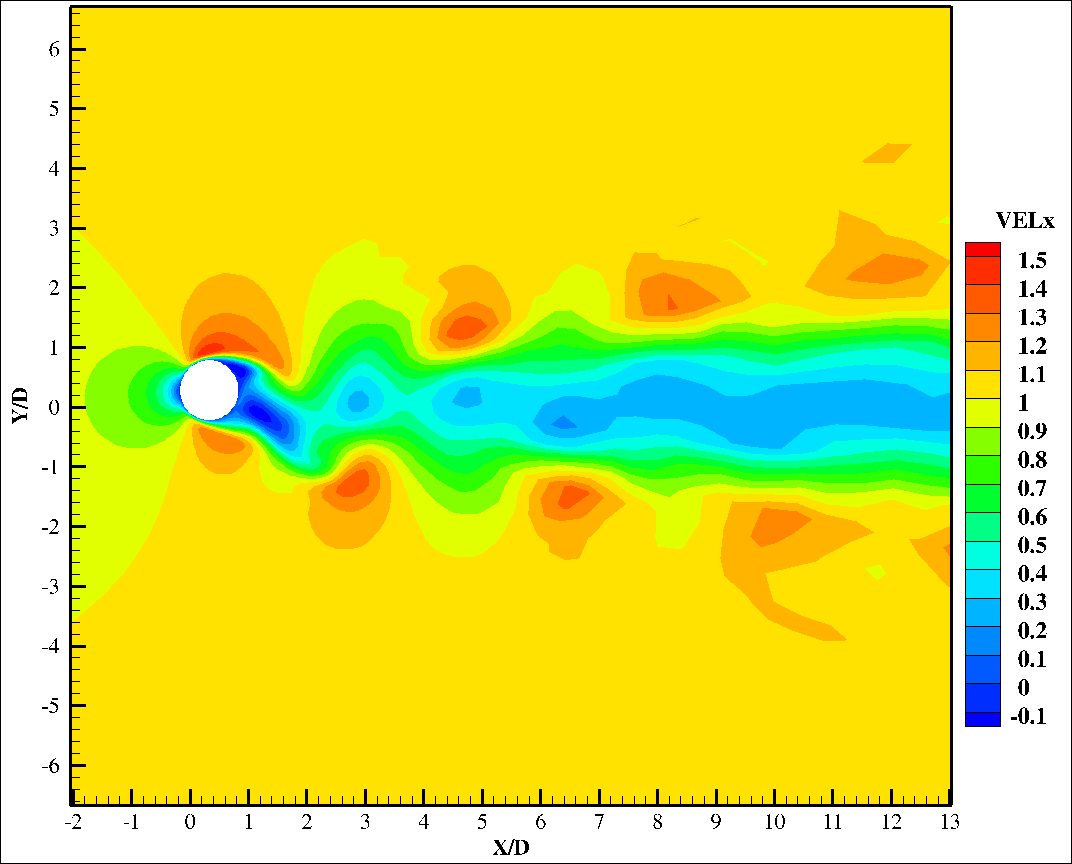
\includegraphics[width=6.5cm]{Sg_1_wor_Vel_153s}}
		\caption{t=153s}
	\end{subfigure}
\caption{Instantaneous velocity contour}
\label{fig:4.6}
\end{figure}

The mean value of drag coefficient $\bar{C_d}$ is calculated to be around 1.72 for all the three under relaxation schemes. The rms value of lift coefficient $C_{l,rms}$ is calculated to be around 0.7. These values are in good concordance with the values of \citet{zhou1999vortex}.

\begin{figure}[H]
\centering
	\begin{subfigure}[t]{7cm}
		\fbox{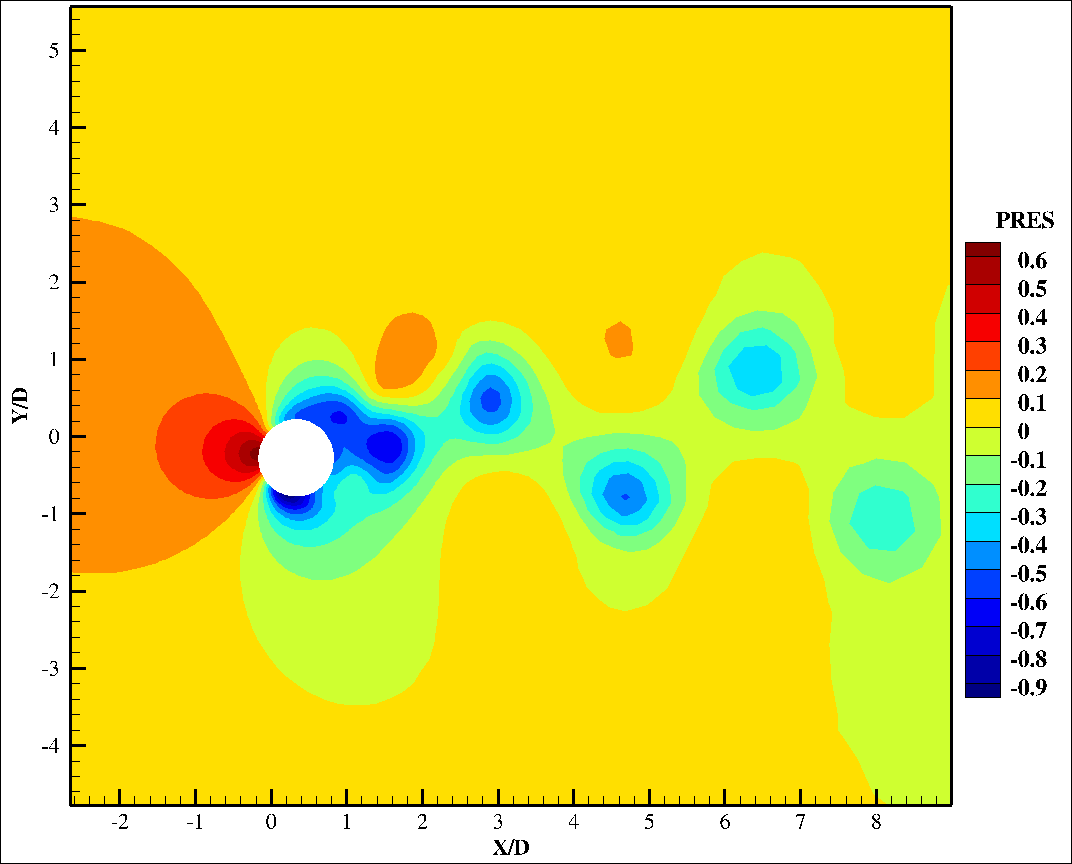
\includegraphics[width=6.5cm]{Sg_1_wor_pres_150_5}}
		\caption{t=150.5s}
	\end{subfigure}
%	\hspace{4cm}
	\begin{subfigure}[t]{7cm}
%		\centering
		\fbox{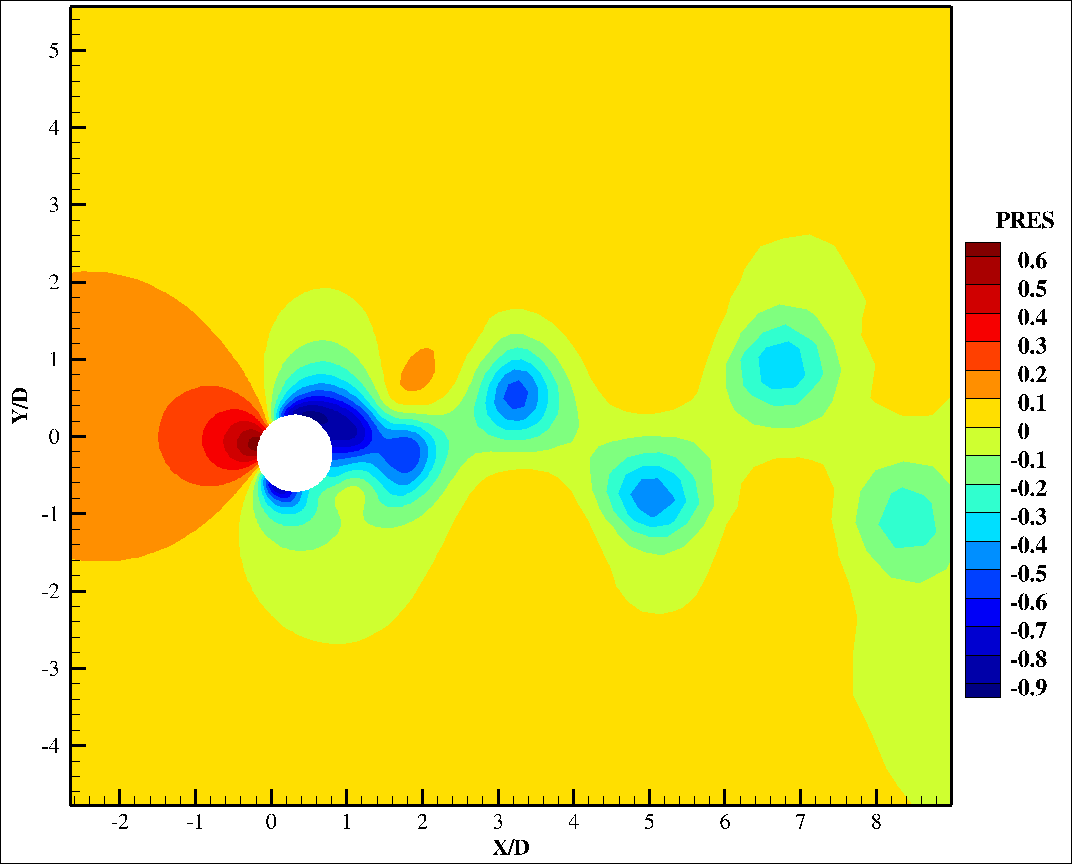
\includegraphics[width=6.5cm]{Sg_1_wor_pres_151}}
		\caption{t=151s}
	\end{subfigure}
	
	\begin{subfigure}[t]{7cm}
		\fbox{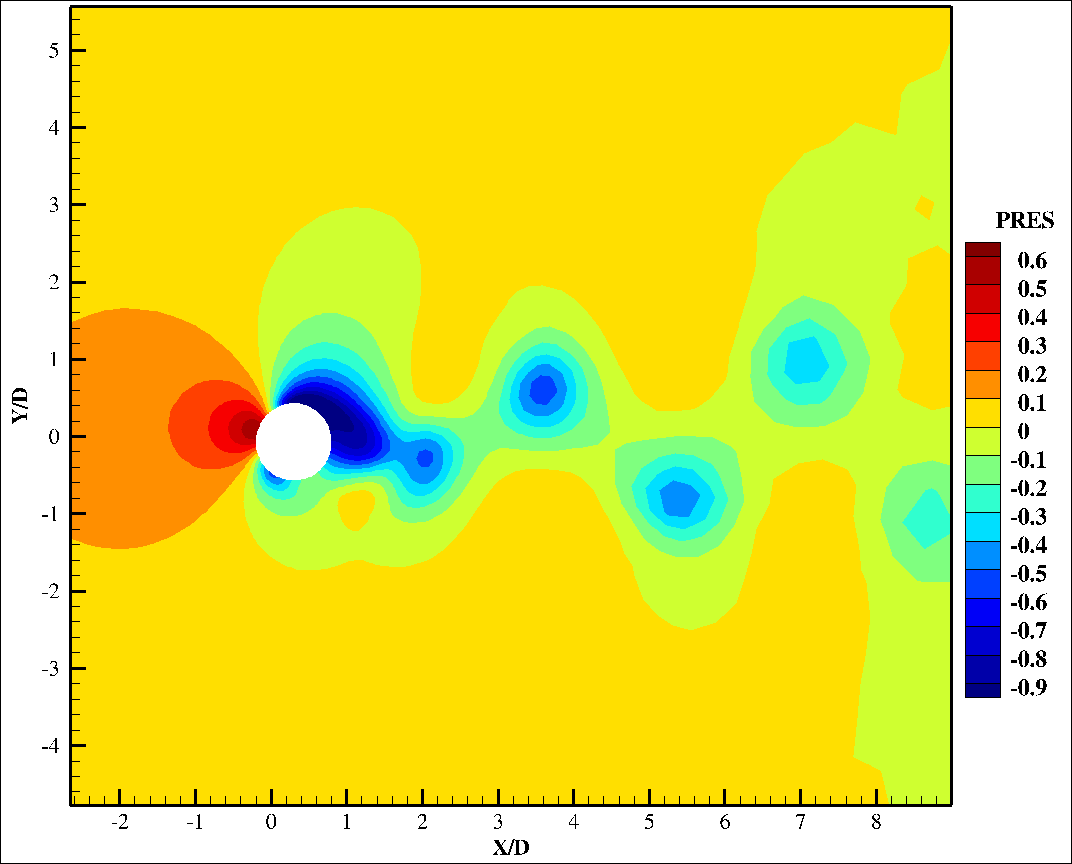
\includegraphics[width=6.5cm]{Sg_1_wor_pres_151_5}}
		\caption{t=151.5s}
	\end{subfigure}
%	\hspace{4cm}
	\begin{subfigure}[t]{7cm}
%		\centering
		\fbox{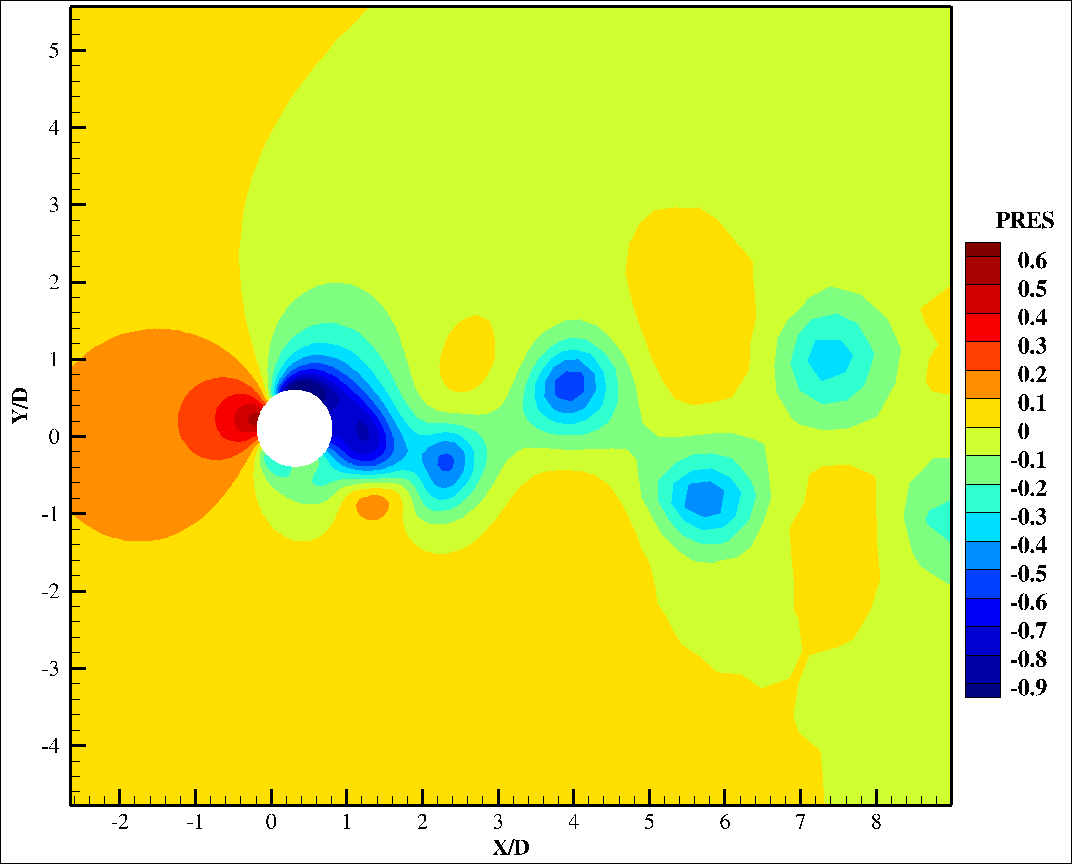
\includegraphics[width=6.5cm]{Sg_1_wor_pres_152}}
		\caption{t=152}
	\end{subfigure}
	
	\begin{subfigure}[t]{7cm}
		\fbox{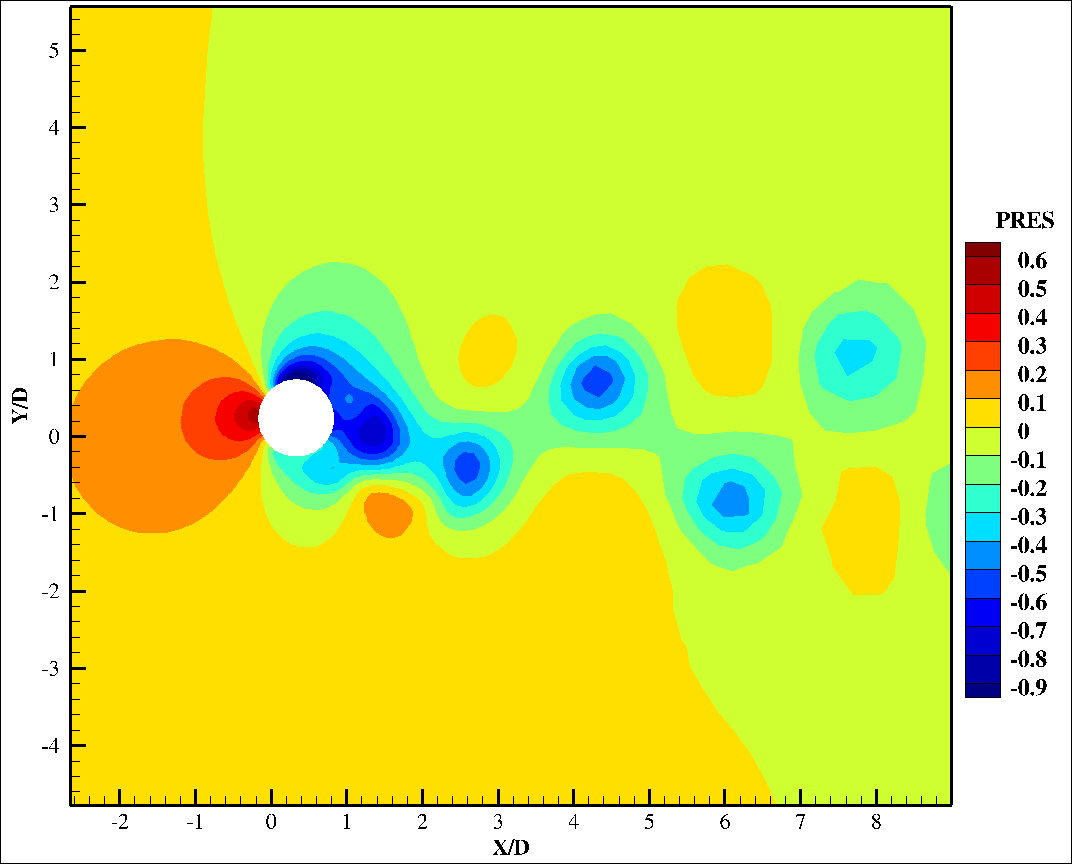
\includegraphics[width=6.5cm]{Sg_1_wor_pres_152_5}}
		\caption{t=152.5}
	\end{subfigure}
%	\hspace{4cm}
	\begin{subfigure}[t]{7cm}
%		\centering
		\fbox{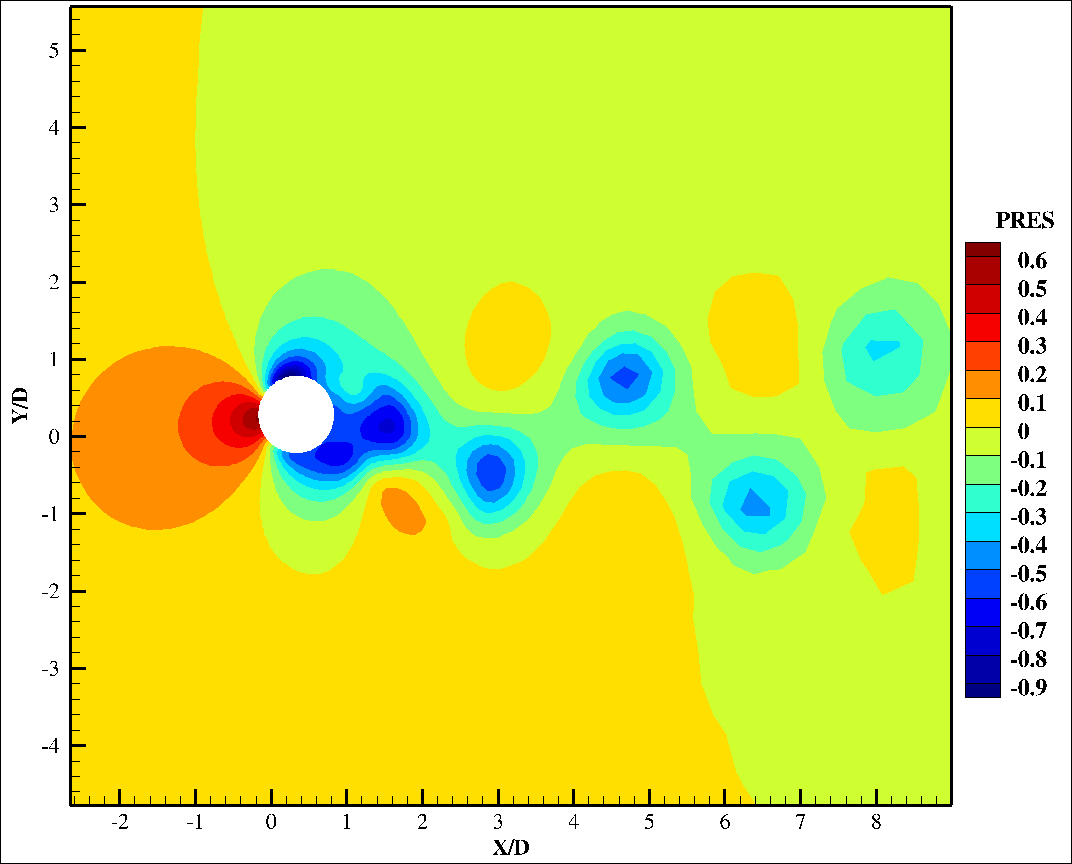
\includegraphics[width=6.5cm]{Sg_1_wor_pres_153}}
		\caption{t=153}
	\end{subfigure}
\caption{Instantaneous pressure contour plots}
\label{fig:4.7}
\end{figure}

In the figure \ref{fig:4.8} the oscillation of the cylinder is quantified and plotted against a certain period of time. As observed in the force coefficient comparison plot, the onset of oscillation for different under relaxation schemes is observed to be varying. The onset of oscillation is at a position $(X/D)_{min}=0.3026, (Y/D)_{min}=-0.2821$ and the transverse oscillation attains a max value of $(Y/D)_{max}=0.2821$ whereas the streamwise oscillation reaches a max distance of $(X/D)_{max}=0.3447$.

\begin{figure}[H]
\centering
\fbox{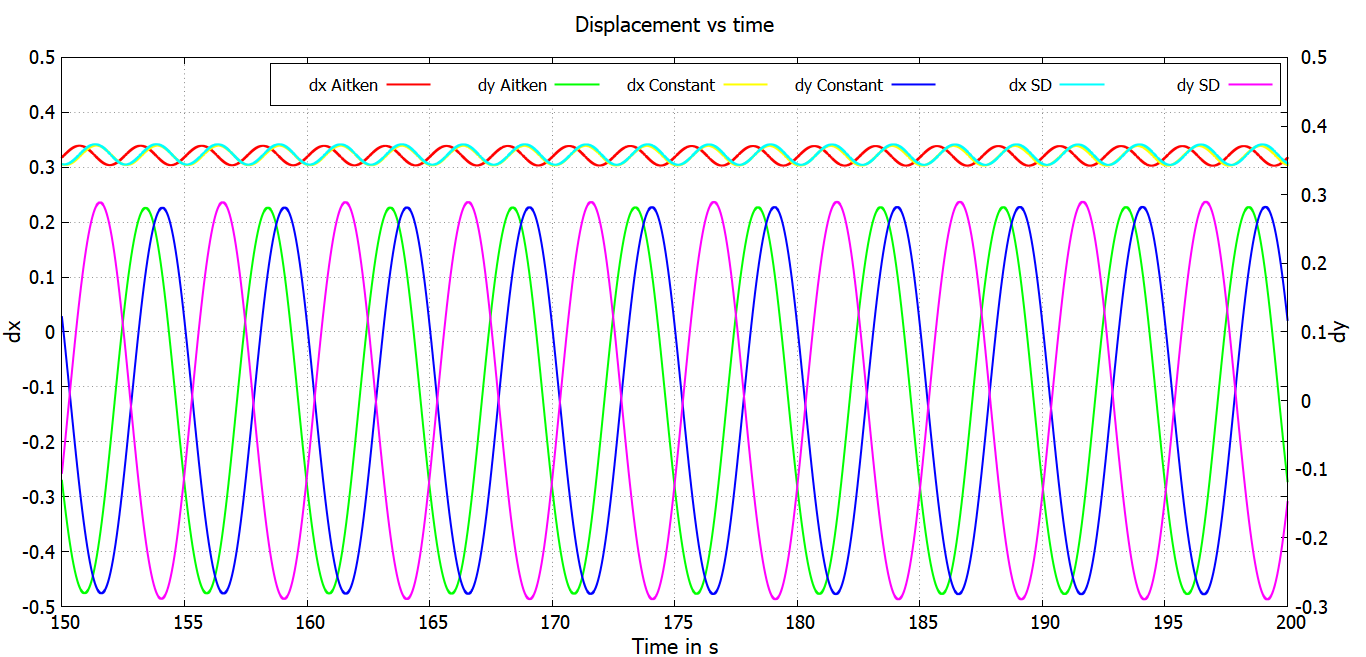
\includegraphics[width=\linewidth]{DC_Sg1_wor}}
\caption{Variation of displacements vs time}
\label{fig:4.8}
\end{figure}

The vortex induced vibration process is a \textit{self limiting process.} According to the study of \citet{griffin1992vortex}, the amplitude of the vibrations could be correlated by Sg. The data examined in the study follow an universal curve. The displacement phase plots appear to have a "figure of 8" shape. The displacement phase plots for the current thesis study is represented in the figure \ref{fig:4.9}. It can be observed that the cylinder oscillations follow the "figure of 8" shape, which is also observed by \citet{zhou1999vortex}. 

\begin{figure}[H]
\centering
\fbox{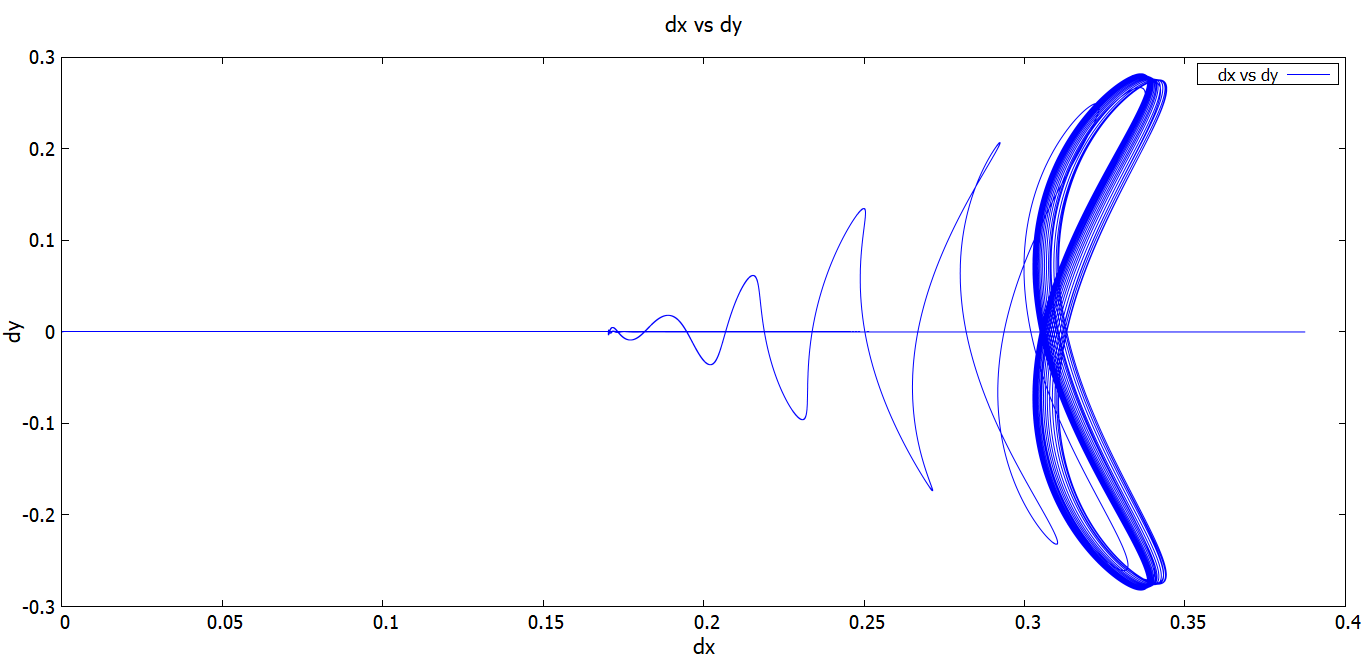
\includegraphics[width=\linewidth]{dxdy_Sg1_wor}}
\caption{Displacement phase plot}
\label{fig:4.9}
\end{figure}

All the quantitative values observed in this simulation study is tabulated and compared with reference values of \citet{zhou1999vortex}. The tabular summary is presented in the table \ref{table:4.6}. The observed values are comparable with the reference values.

% Table generated by Excel2LaTeX from sheet 'M1_Sg1'
\begin{table}[htbp]
  \centering
   \begin{tabular}{|l|c|c|c|c|c|c|c|}
    \hline
    \multicolumn{1}{|c|}{\multirow{2}[4]{*}{Simulation cases}} & \multicolumn{7}{c|}{Values} \\
\cline{2-8}          & $(X/D)_{min}$ & $(X/D)_{max}$ & $(Y/D)_{min}$ & $(Y/D)_{max}$ & $\bar{C_d}$   & $C_{l,rms}$ & $2Y_{rms}/D$ \\
    \hline
    Constant & 0.3027 & 0.3447 & -0.2825 & 0.2825 & 1.7253 & 0.7   & 0.3992 \\
    \hline
    Aitken & 0.3026 & 0.3445 & -0.2821 & 0.2821 & 1.7244 & 0.6998 & 0.3987 \\
    \hline
    SD    & 0.3026 & 0.3445 & -0.2811 & 0.2811 & 1.7248 & 0.6998 & 0.3973 \\
    \hline
    Zhou et. al. & 0.2818 & 0.38  & -0.27 & 0.28  & 1.66  & 0.65  & 0.34 \\
    \hline
    \end{tabular}%
    \caption{Tabular summary of quantitative values observed for case 1 without a flow restart file}
  \label{table:4.6}%
\end{table}%

\subsubsection{With a flow restart file}
For this simulation, the initial conditions are used from the rigid cylinder case. The simulations were started at a physical time of 200s, and were performed for nearly 50 vortex shedding cycles. 

The results of the simulation is presented in this section. In figure \ref{fig:4.10} the force coefficients ($C_d$) and ($C_l$) are compared and visualized for an approximate period of 10 oscillations of the cylinder in the transverse direction of the flow. It could be observed that the onset of oscillations are happening exactly at the same time irrespective of the relaxation schemes. This could be attributed to the fact that the initial conditions are the same in each case and the system is in equilibrium. The mean and rms values of the coefficients are calculated to be $\bar{C_d} = 1.72$ and $C_{l,rms} = 0.70$ respectively, which is exactly similar to the values observed with the non-restart simulation.

\begin{figure}[H]
\centering
\fbox{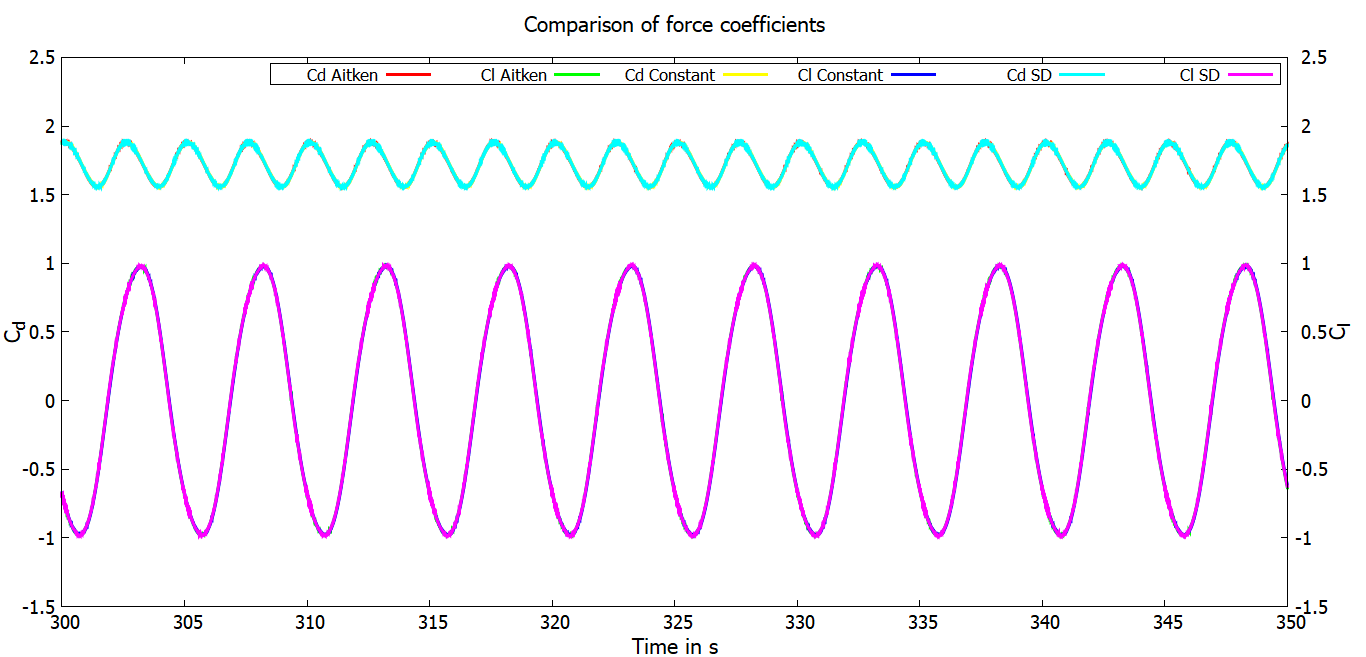
\includegraphics[width=\linewidth]{FC_Sg1_wr}}
\caption{Variation of Drag and Lift coefficients for case 1 with a flow restart file}
\label{fig:4.10}
\end{figure}

In the figure \ref{fig:4.11} the variation of displacements over time is studied for the same period of about 5 oscillations of the cylinder. The onset of oscillation is observed at a position $(X/D)_{min}=0.30, (Y/D)_{min}=-0.28$ and the transverse oscillation attains a max value of $(Y/D)_{max}=0.28$ whereas the streamwise oscillation reaches a max distance of $(X/D)_{max}=0.34$. These values are similar to the simulation with the non-restart case. It can be observed that all three relaxation schemes has the same values and the oscillations are also identical.

\begin{figure}[H]
\centering
\fbox{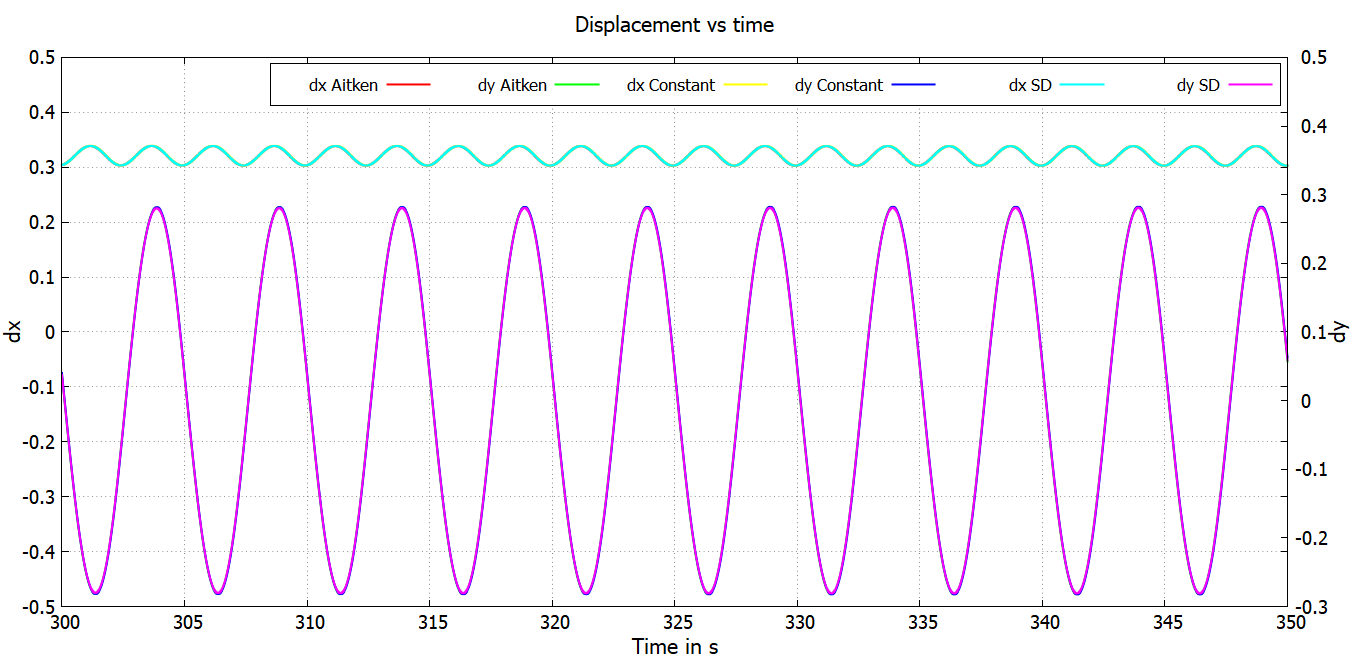
\includegraphics[width=\linewidth]{DC_Sg1_wr}}
\caption{Variation of displacements vs time}
\label{fig:4.11}
\end{figure}

The displacement phase plot for this simulation is represented in the figure \ref{fig:4.12}. It can be observed that the supposed "figure of 8" shape has been replicated in this simulation as well. However, the equilibrium position of the vibration in the streamwise direction is not zero, which was the case with previous simulation result. 

The equilibrium position is comparable to the results observed by \citet{zhou1999vortex}. This could be attributed to the initial conditions, which affects the equilibrium position of vibration. The observed quantitative values are summarized in the table \ref{table:4.7}. The values observed are identical to the case with non-restart and comparable to the reference values.

\begin{figure}[H]
\centering
\fbox{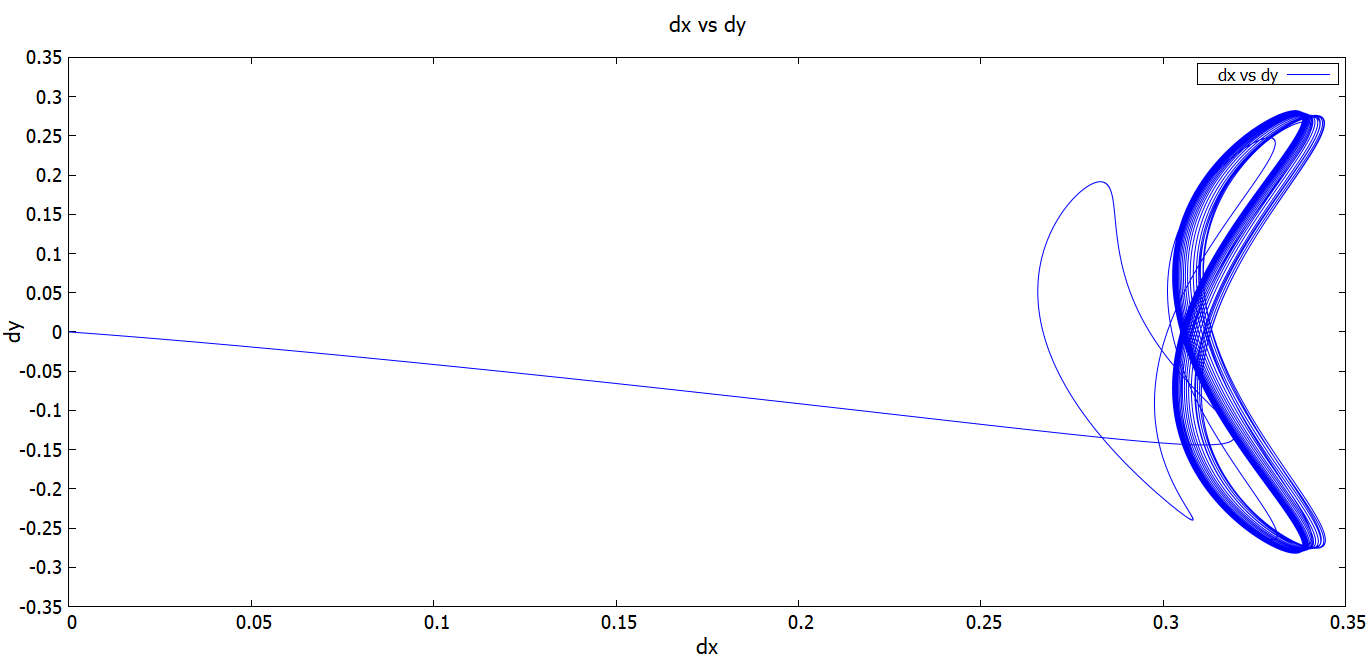
\includegraphics[width=\linewidth]{dxdy_Sg1_wr}}
\caption{Displacement phase plot}
\label{fig:4.12}
\end{figure}

\begin{table}[htbp]
  \centering
   \begin{tabular}{|l|c|c|c|c|c|c|c|}
    \hline
    \multicolumn{1}{|c|}{\multirow{2}[4]{*}{Simulation cases}} & \multicolumn{7}{c|}{Values} \\
\cline{2-8}          & $(X/d)_{min}$ & $(X/d)_{max}$ & $(Y/d)_{min}$ & $(Y/d)_{max}$ & $\bar{C_d}$  & $C_{l,rms}$ & $2Y_{rms}/D$ \\
    \hline
    Constant & 0.3027 & 0.344 & -0.2825 & 0.2825 & 1.723 & 0.7009 & 0.3994 \\
    \hline
    Aitken & 0.3026 & 0.3433 & -0.2821 & 0.2821 & 1.7231 & 0.7023 & 0.3989 \\
    \hline
    SD    & 0.304 & 0.3446 & -0.2898 & 0.2898 & 1.7335 & 0.7104 & 0.4005 \\
    \hline
    Zhou et. al. & 0.2818 & 0.38  & -0.27 & 0.28  & 1.66  & 0.65  & 0.34 \\
    \hline
    \end{tabular}%
    \caption{Tabular summary of quantitative values observed for case 1 with a flow restart file}
  \label{table:4.7}%
\end{table}%

\subsubsection{Study of acceleration parameters}

In the simulations conducted for the case-1 with and without restart, the acceleration of the implemented adaptive relaxation schemes has been studied. This section deals with the discussion of the observations made during the study. Two major factors are studied and used as a source of comparison between the cases.

\begin{enumerate}[(i)]
\item Average number of FSI sub-iterations per time step during the solution (${sub-iter}_{mean}$)
\item Average time taken per time step during the solution (${\bar{t}} per ts$), where ts is time step.
\end{enumerate}

All three schemes have been simulated for a total of around 50 vortex shedding cycles, (physical time scale of approximately 256s). The observed quantities are quantified in the table below.

% Table generated by Excel2LaTeX from sheet 'M1_Sg1'
\begin{table}[htbp]
  \centering
   \begin{tabular}{|l|c|c|c|c|}
    \hline
    \multicolumn{1}{|c|}{\multirow{2}[4]{*}{Simulation cases}} & \multicolumn{4}{c|}{Acceleration parameters} \\
\cline{2-5}          & ${sub-iter}_{max}$ & ${sub-iter}_{min}$ & ${sub-iter}_{mean}$ & ${\bar{t}} per ts$ in s \\
    \hline
    Constant & 22    & 11    & 13    & 0.44 \\
    \hline
    Aitken & 25    & 3     & 8     & 0.19 \\
    \hline
    SD    & 19    & 11    & 9     & 0.8 \\
    \hline
    \end{tabular}%
   \caption{Acceleration parameters observed during the simulation of case 1}
  \label{table:4.8}%
\end{table}%

As expected \textit{Aitken} relaxation scheme offers the best results, with an average time per time step of 0.19s, which is twice as efficient as the current implementation of constant URF scheme. However, the method of \textit{Steepest Descent} offers worse results. It is only nearly half as fast compared to the current version, even though the average number of sub-iterations is reduced by 2 when compared with \textit{Constant URF} implementation. This is because, the \textit{Steepest Descent} method requires an additional run of the FSI solver during each time step in order to calculate the Jacobian matrix. 

\subsection{Results for case 2: M=1 and Sg=0.1}
In this section the results for the case with a mass ratio M=1 and damping coefficient Sg=0.1 is presented. The simulation results of this case with various parameters just like above is presented and discussed in this section. 

\subsubsection{Results for case 2 without a restart file}
In this simulation, the cylinder is suspended elastically from the start of simulation. The system characteristics are studied and discussed in this sub-section. In the figures \ref{fig:4.13} and \ref{fig:4.14} the velocity and pressure plots for a time period of approximately one oscillation of the cylinder is presented. From these plots, it could be observed that the oscillations are much erratic than the case 1 with a damping coefficient of Sg=1. The vortices are shed rapidly and it can be observed that the shedding takes place in the middle of the oscillation cycle. The vortices stream is much more chaotic in the flow downstream of the cylinder. This is due to the fact that the cylinder is comparatively free to oscillate due to the lesser damping factor considered. 

The solver settings used for this simulation is tabulated in the table \ref{table:4.9}. The values of  physical properties such as stiffness coefficient k and damping factor d[kg/s] is represented in the table.

\begin{table}[htbp]
  \centering
   \begin{tabular}{|l|l|}
    \hline
    Time integration & 3 step Runge-Kutta \\
    \hline
    Number of time steps & \multicolumn{1}{p{8.645em}|}{300000\newline{}($\approx$ 50 vortex shedding cycles)} \\
    \hline
    M     & 1 \\
    \hline
    Sg    & 0.01 \\
    \hline
    k[N/m]     & 2.6802 \\
    \hline
    d[kg/s]     & 0.3331 \\
    \hline
    \end{tabular}%
  \caption{Solver settings for the simulation}
  \label{table:4.9}%
\end{table}%

\begin{figure}[H]
\centering
	\begin{subfigure}[t]{7cm}
		\fbox{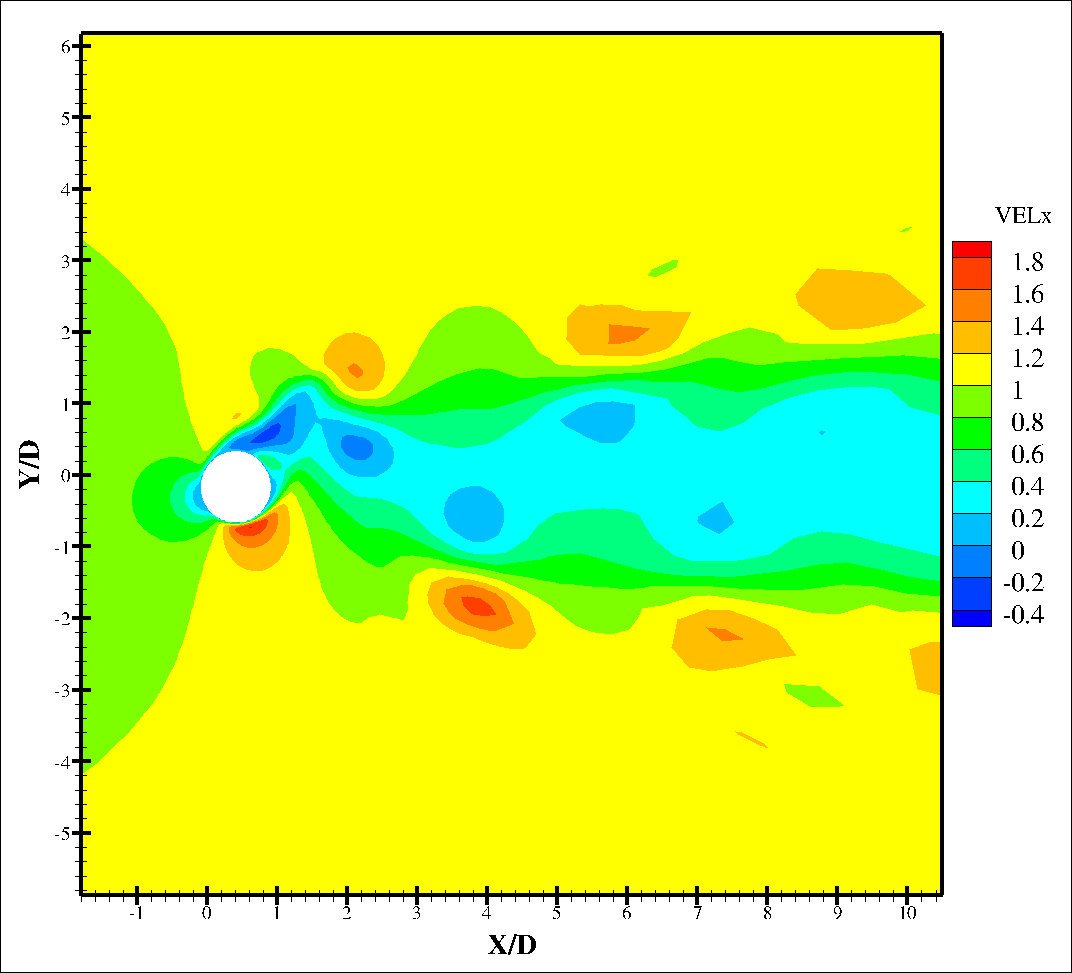
\includegraphics[width=6.5cm]{Sg_01_v_150_5}}
		\caption{t=150.5s}
	\end{subfigure}
%	\hspace{4cm}
	\begin{subfigure}[t]{7cm}
%		\centering
		\fbox{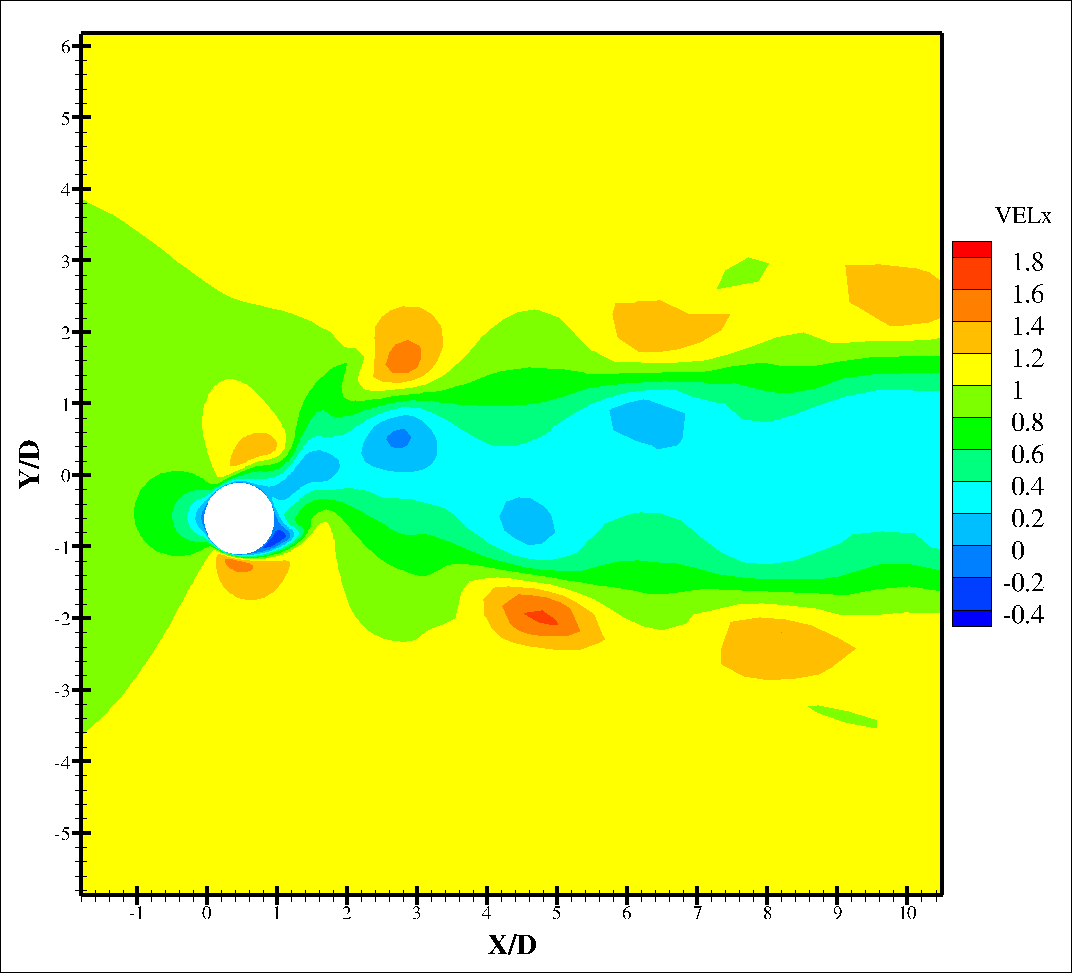
\includegraphics[width=6.5cm]{Sg_01_v_151}}
		\caption{t=151s}
	\end{subfigure}
	
	\begin{subfigure}[t]{7cm}
		\fbox{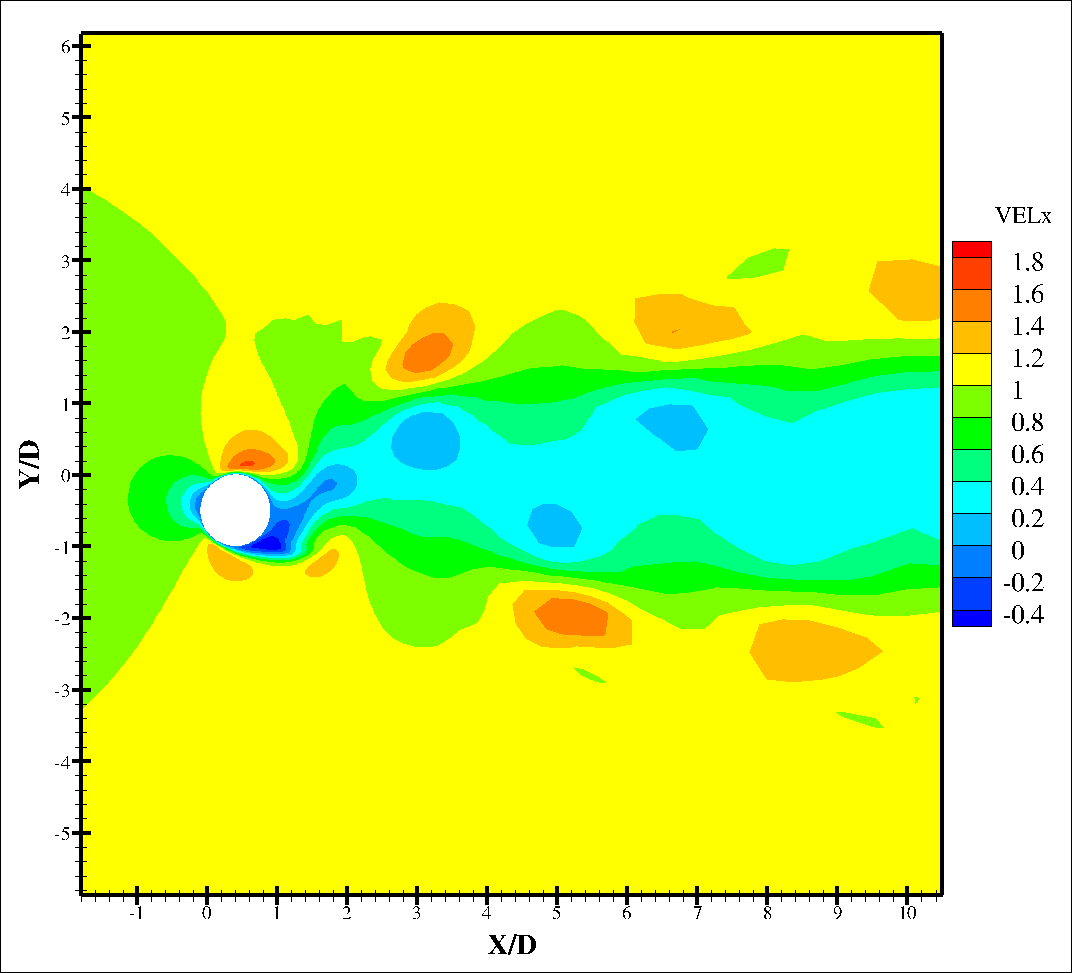
\includegraphics[width=6.5cm]{Sg_01_v_151_5}}
		\caption{t=151.5s}
	\end{subfigure}
%	\hspace{4cm}
	\begin{subfigure}[t]{7cm}
%		\centering
		\fbox{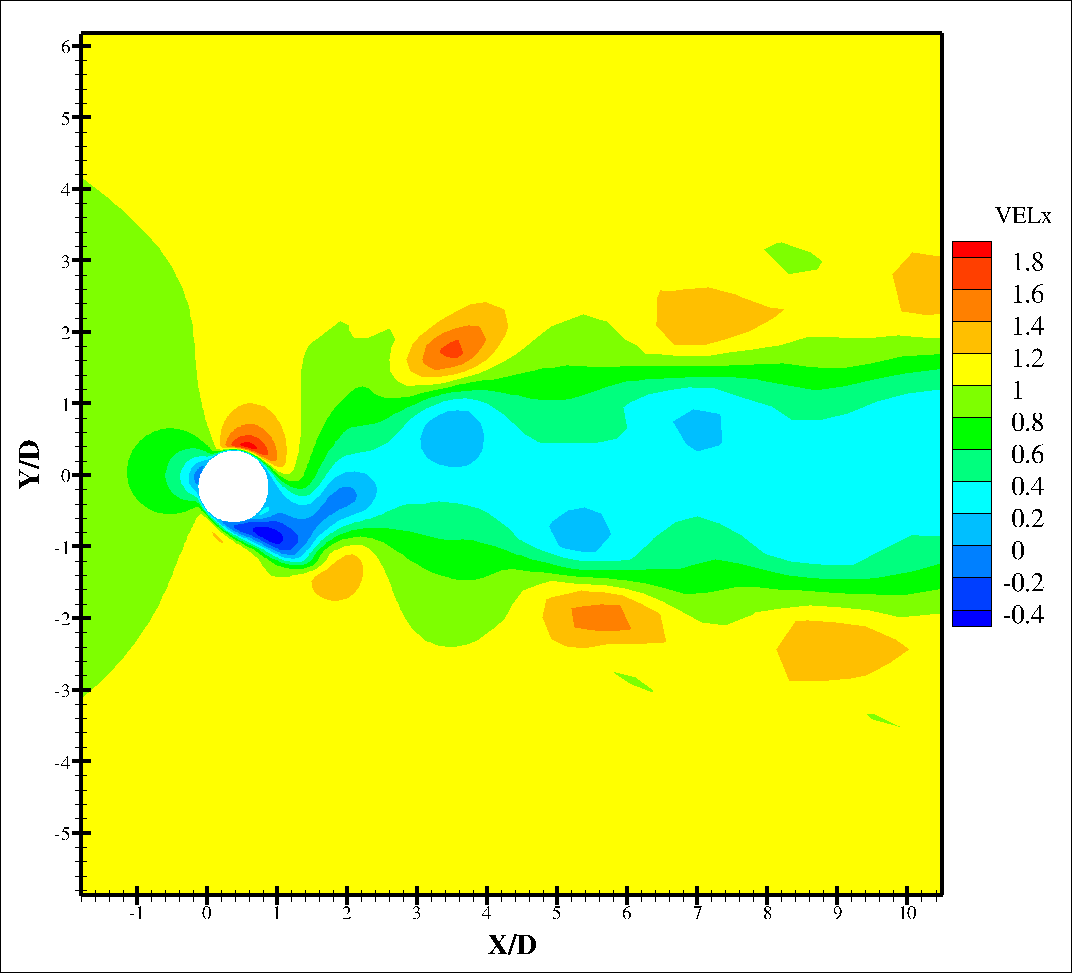
\includegraphics[width=6.5cm]{Sg_01_v_152}}
		\caption{t=152s}
	\end{subfigure}
	
	\begin{subfigure}[t]{7cm}
		\fbox{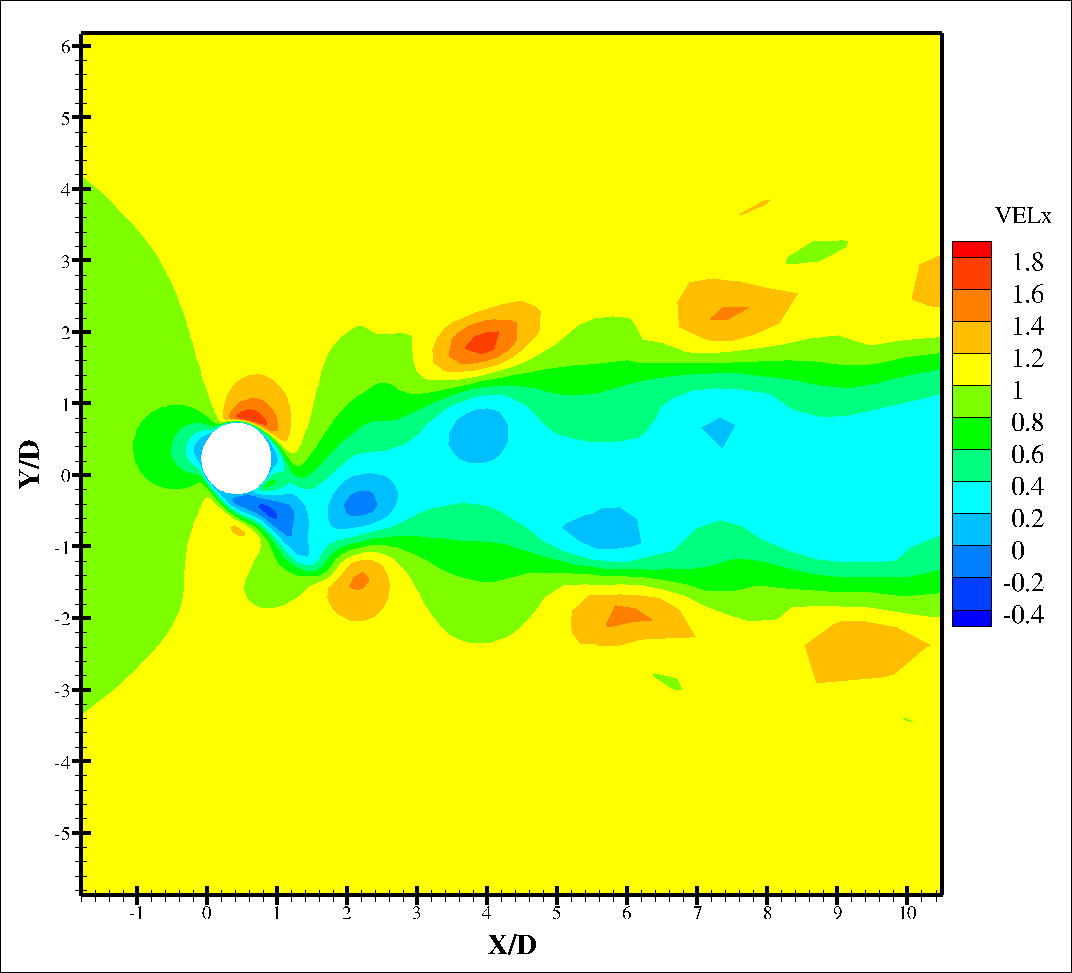
\includegraphics[width=6.5cm]{Sg_01_v_152_5}}
		\caption{t=152.5s}
	\end{subfigure}
%	\hspace{4cm}
	\begin{subfigure}[t]{7cm}
%		\centering
		\fbox{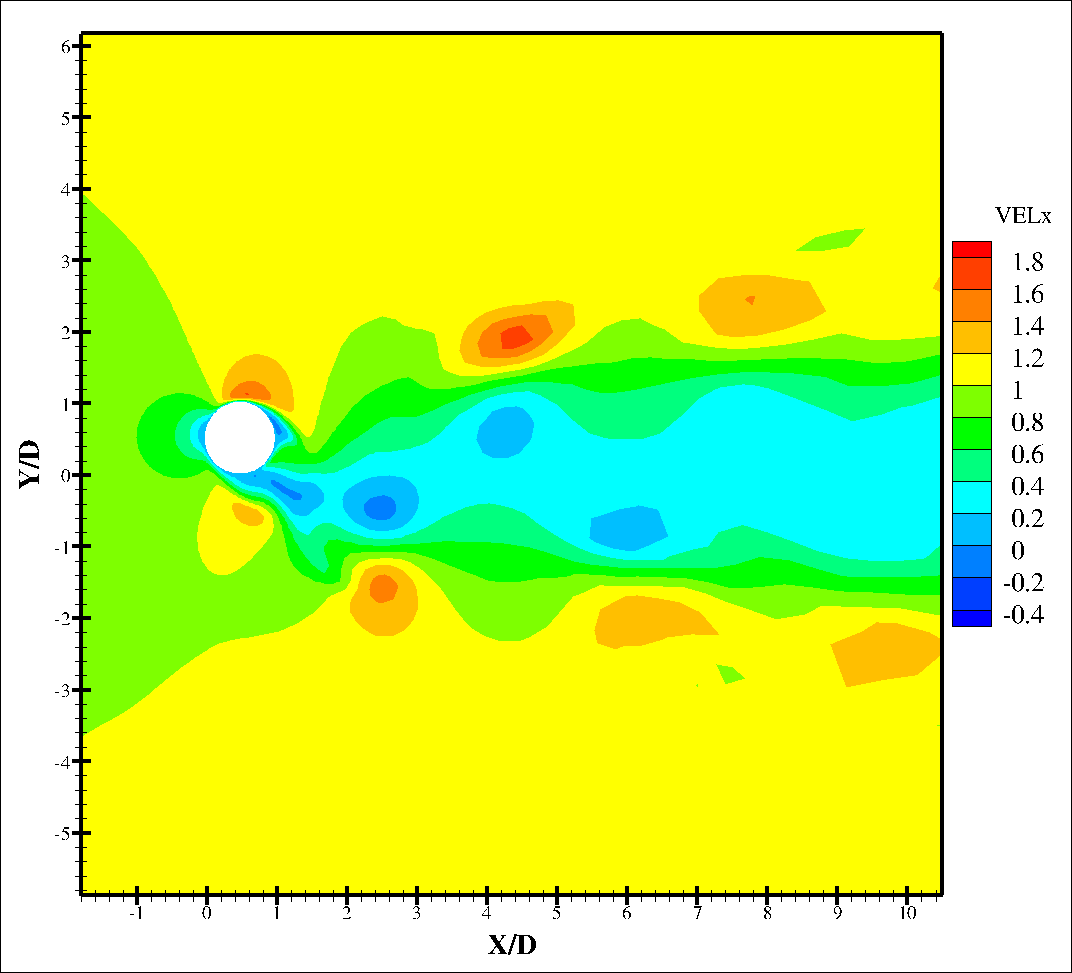
\includegraphics[width=6.5cm]{Sg_01_v_153}}
		\caption{t=153s}
	\end{subfigure}
\caption{Instantaneous velocity contour}
\label{fig:4.13}
\end{figure}

\begin{figure}[H]
\centering
	\begin{subfigure}[t]{7cm}
		\fbox{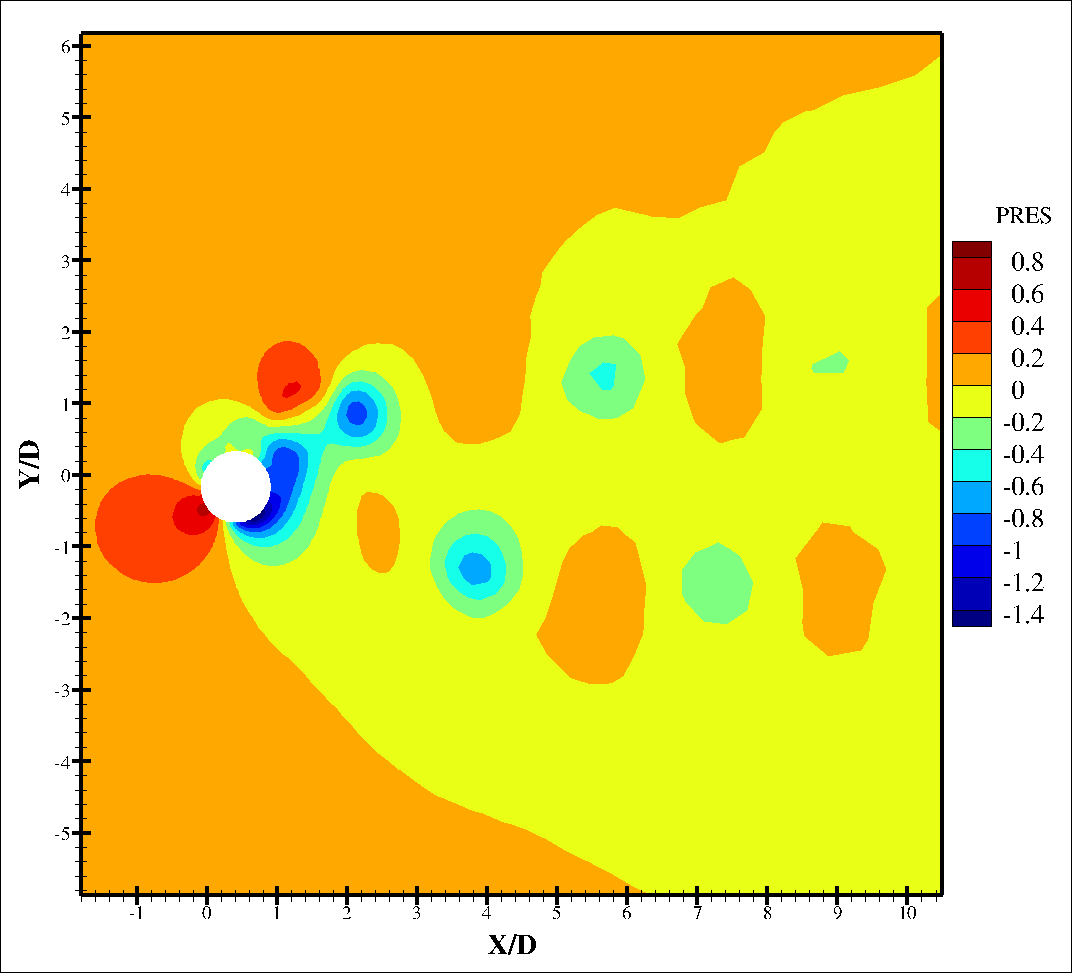
\includegraphics[width=6.5cm]{Sg_01_wor_p_150_5}}
		\caption{t=150.5s}
	\end{subfigure}
%	\hspace{4cm}
	\begin{subfigure}[t]{7cm}
%		\centering
		\fbox{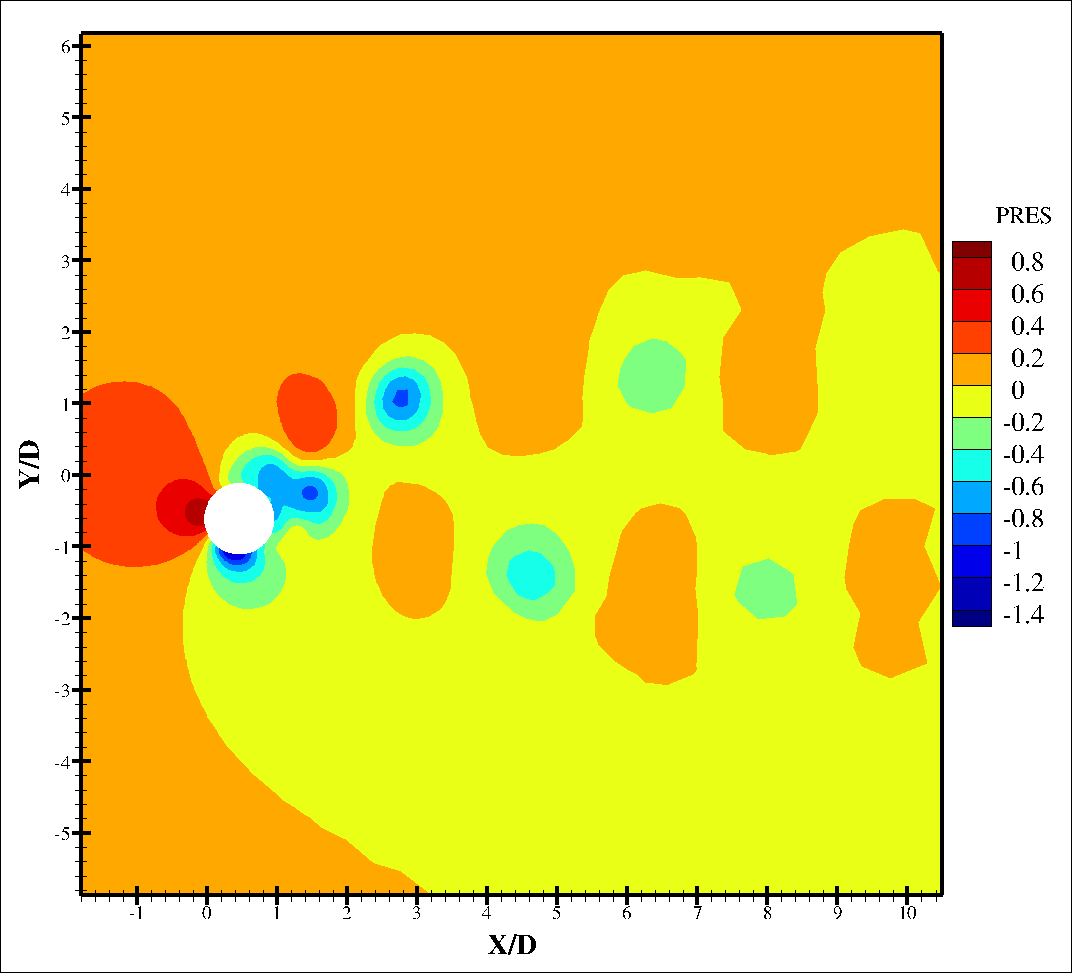
\includegraphics[width=6.5cm]{Sg_01_wor_p_151}}
		\caption{t=151s}
	\end{subfigure}
	
	\begin{subfigure}[t]{7cm}
		\fbox{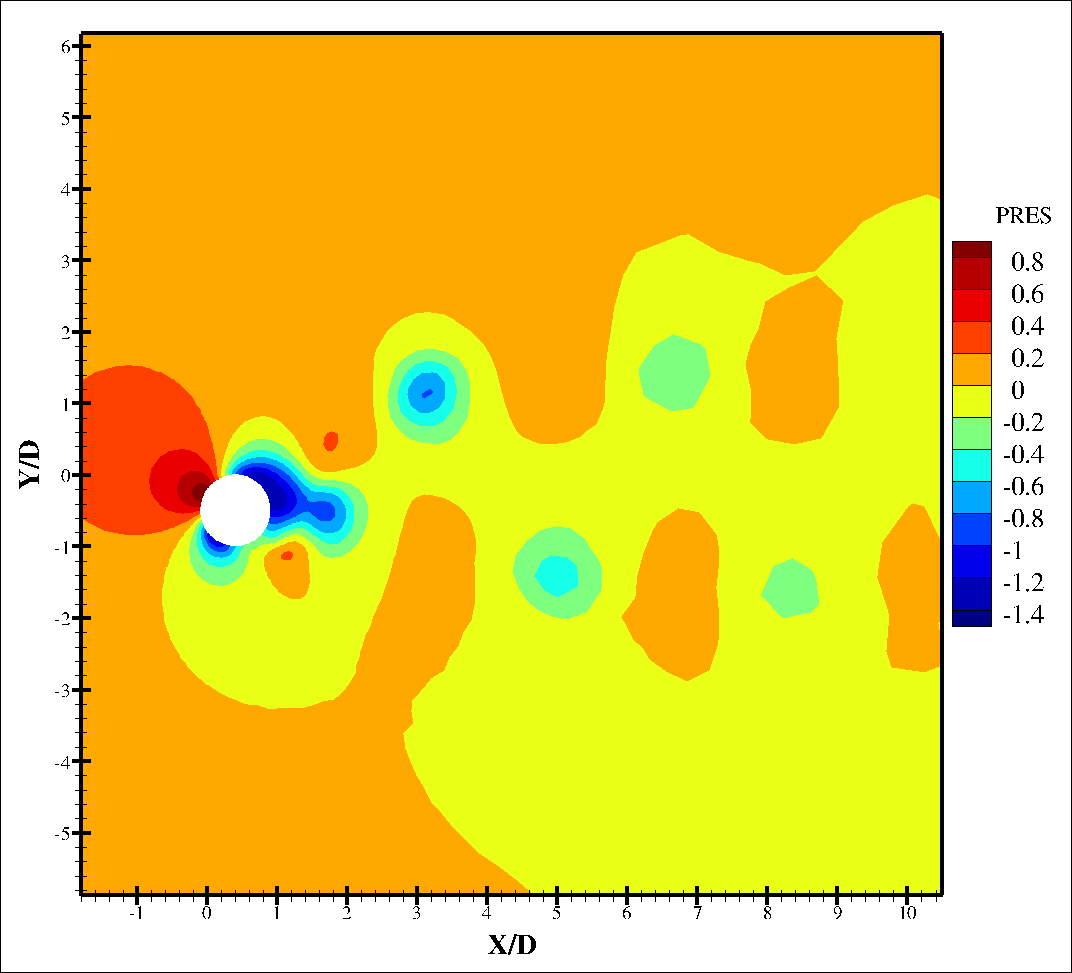
\includegraphics[width=6.5cm]{Sg_01_wor_p_151_5}}
		\caption{t=151.5s}
	\end{subfigure}
%	\hspace{4cm}
	\begin{subfigure}[t]{7cm}
%		\centering
		\fbox{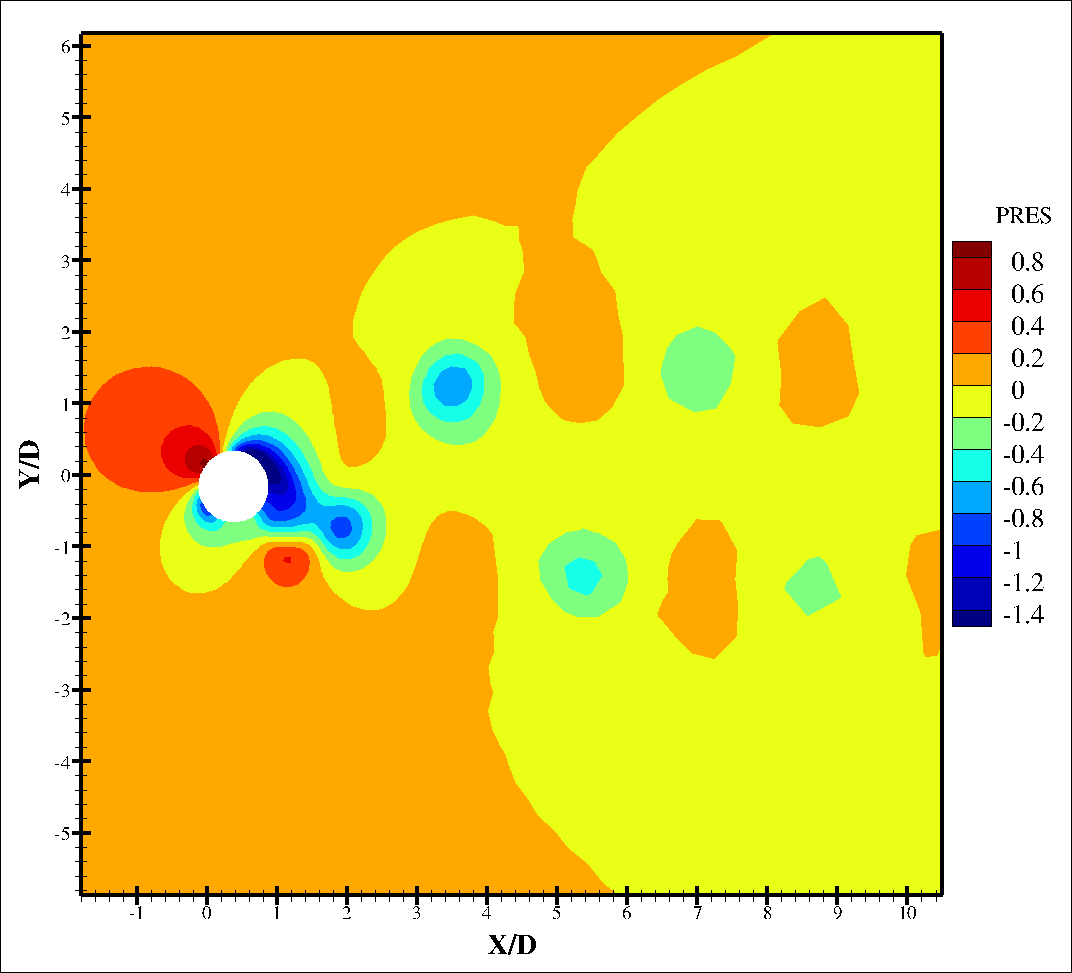
\includegraphics[width=6.5cm]{Sg_01_wor_p_152}}
		\caption{t=152s}
	\end{subfigure}
	
	\begin{subfigure}[t]{7cm}
		\fbox{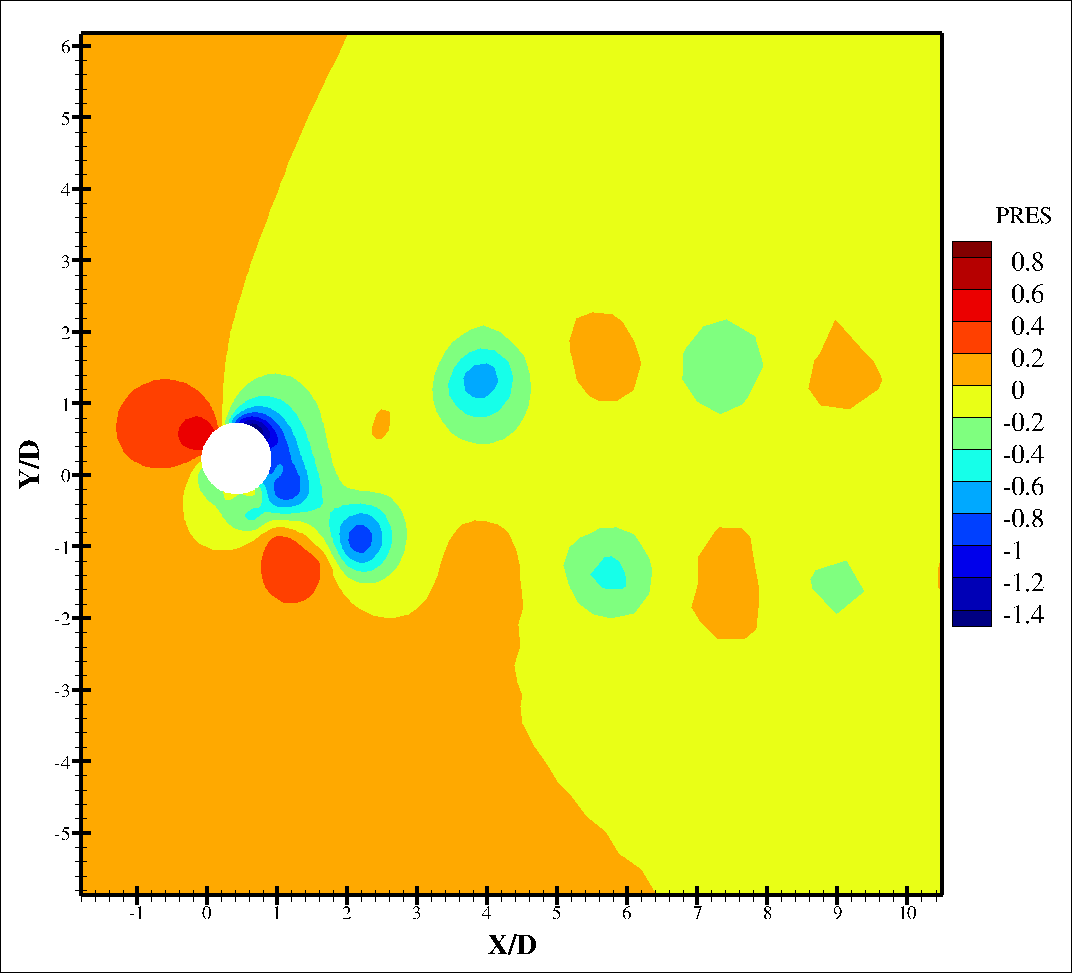
\includegraphics[width=6.5cm]{Sg_01_wor_p_152_5}}
		\caption{t=152.5s}
	\end{subfigure}
%	\hspace{4cm}
	\begin{subfigure}[t]{7cm}
%		\centering
		\fbox{\includegraphics[width=6.5cm]{Sg_01_wor_p_153}}
		\caption{t=153s}
	\end{subfigure}
\caption{Instantaneous pressure contour}
\label{fig:4.14}
\end{figure}

In the figure \ref{fig:4.15} the variation of force coefficients $C_d$ and $C_l$ is plotted for a period of approximately 10 oscillations of the cylinder. Once again, the onset of the oscillations are little different for each of the relaxation schemes. In the figure \ref{fig:4.16} the variation of displacements is represented for the same time period. The onset of oscillation is observed at a position $(X/D)_{min}=0.37, (Y/D)_{min}=-0.61$ and the transverse oscillation attains a max value of $(Y/D)_{max}=0.61$ whereas the streamwise oscillation reaches a max distance of $(X/D)_{max}=0.48$. 

\begin{figure}[H]
\centering
\fbox{\includegraphics[width=\linewidth]{FC_Sg01_wor}}
\caption{Variation of Drag and Lift coefficients for case 2 without a flow restart file}
\label{fig:4.15}
\end{figure}

\begin{figure}[H]
\centering
\fbox{\includegraphics[width=\linewidth]{DC_Sg01_wor}}
\caption{Variation of displacements vs time}
\label{fig:4.16}
\end{figure}

The displacement phase plot is represented in the figure \ref{fig:4.17}. The "figure of 8" shape is maintained with the equilibrium position of the displacement in the streamline direction observed to be at the mean position of oscillation.

\begin{figure}[H]
\centering
\fbox{\includegraphics[width=\linewidth]{dxdy_Sg01_wor}}
\caption{Displacement phase plot}
\label{fig:4.17}
\end{figure} 

The values are summarized in the table \ref{table:4.10}. The main characteristics $\bar{C_d}$ and $C_{l,rms}$ are in good agreement with the values observed by \citet{zhou1999vortex}. The difference in other values could be due to the different simulation setup and the usage of solver.

\begin{table}[htbp]
  \centering
   \begin{tabular}{|l|c|c|c|c|c|c|c|}
    \hline
    \multicolumn{1}{|c|}{\multirow{2}[4]{*}{Simulation cases}} & \multicolumn{7}{c|}{Values} \\
\cline{2-8}          & $(X/d)_{min}$ & $(X/d)_{max}$ & $(Y/d)_{min}$ & $(Y/d)_{max}$ & $\bar{C_d}$  & $C_{l,rms}$ & $2Y_{rms}/D$ \\
    \hline
    Constant & 0.3732 & 0.4779 & -0.6111 & 0.6111 & 2.2588 & 0.862 & 0.8655 \\
    \hline
    Aitken & 0.3734 & 0.4741 & -0.611 & 0.611 & 2.2575 & 0.8632 & 0.8641 \\
    \hline
    SD    & 0.3775 & 0.4788 & -0.6255 & 0.6245 & 2.2966 & 0.8684 & 0.8844 \\
    \hline
    Zhou et. al. & 0.28 & 0.5 & -0.57 & 0.56 & 2.06 & 0.84 & 0.75 \\
    \hline
    \end{tabular}%
    \caption{Tabular summary of quantitative values observed for case 2 without a flow restart file}
  \label{table:4.10}%
\end{table}%

\subsubsection{Results for case 2 with a restart file}

This section deals with the results and discussion of the simulation of the case 2 with a flow restart file. This study of with and without flow restart files is conducted to study the effect of initial conditions on the vibration response of the cylinder. In the figure \ref{fig:4.18}, the force comparison plot is represented for a period of 10 oscillations of the cylinder. It could be observed that the $C_d$ has an interesting pattern of oscillation. It has been observed that there is an alternating peak point of oscillation along the streamwise direction. The oscillations along the streamwise direction is continuous with alternating peaks in each cycle of oscillation.

\begin{figure}[H]
\centering
\fbox{\includegraphics[width=\linewidth]{FC_Sg01_wr}}
\caption{Variation of Drag and Lift coefficients for case 2 with a flow restart file}
\label{fig:4.18}
\end{figure}

In the figure \ref{fig:4.19}, the displacement variation of the cylinder is represented. It could be observed that in successive oscillations, the peak displacement along the streamwise direction alternates between 0.5 and 0.45. This pattern is not observed in the previous simulation which was without a restart file. The difference in the pattern observed could be due to the differing initial conditions.  

\begin{figure}[H]
\centering
\fbox{\includegraphics[width=\linewidth]{DC_Sg01_wr}}
\caption{Variation of displacements vs time}
\label{fig:4.19}
\end{figure}

As observed in the case 1 (M=1,Sg=1), the displacement phase plot is observed to follow the same pattern. The equilibrium position of the mean streamwise displacement is not along the zero position. The displacement phase plot is represented in the \ref{fig:4.20}.

\begin{figure}[H]
\centering
\fbox{\includegraphics[width=\linewidth]{dxdy_Sg01_wr}}
\caption{Displacement phase plot}
\label{fig:4.20}
\end{figure}

The pressure variation near the cylinder surface, downstream and in the wake region is studied for a period of one oscillation has been studied for both the simulations with and without restart file. The location of the line along which the pressure values is plotted is shown in the figure %\ref{fig:4.21}. 
The pattern of pressure variation differs between the simulated cases. This maybe due to the effect of the wake region. This comparison plot is represented in the figure \ref{fig:4.22}. The wake region is well established in the simulation with the restart file during the start of the simulation.

%%%%%%%%%%%%%%%Insert figure with line represented along the cylinder%%%

\begin{figure}[H]
\centering
	\begin{subfigure}[t]{7cm}
		\fbox{\includegraphics[width=6.5cm]{PP_wor}}
		\caption{Without a restart file}
	\end{subfigure}
%	\hspace{4cm}
	\begin{subfigure}[t]{7cm}
%		\centering
		\fbox{\includegraphics[width=6.5cm]{PP_wr}}
		\caption{With a restart file}
	\end{subfigure}
\caption{Pressure variation along the represented line for case 2 without and with a restart file}
\label{fig:4.22}
\end{figure}

In the table \ref{table:4.11}, the observed values are tabulated and compared with the reference values. The min and max values of displacement are different when compared with the simulation case without a restart file. Whereas the mean and rms values of force coefficients are comparable and in good agreement with the reference values.

\begin{table}[htbp]
  \centering
   \begin{tabular}{|l|c|c|c|c|c|c|c|}
    \hline
    \multicolumn{1}{|c|}{\multirow{2}[4]{*}{Simulation cases}} & \multicolumn{7}{c|}{Values} \\
\cline{2-8}          & $(X/d)_{min}$ & $(X/d)_{max}$ & $(Y/d)_{min}$ & $(Y/d)_{max}$ & $\bar{C_d}$  & $C_{l,rms}$ & $2Y_{rms}/D$ \\
    \hline
	Constant  & 0.3162 & 0.5163 & -0.6333 & 0.5967 & 2.245 & 0.8952 & 0.8653 \\
    \hline
    Aitken  & 0.3277 & 0.5162 & -0.6288 & 0.5971 & 2.2469 & 0.8892 & 0.8657 \\
    \hline
    SD    & 0.3209 & 0.5175 & -0.6312 & 0.5985 & 2.2484 & 0.8945 & 0.8685 \\
    \hline
    Zhou et. al. & 0.28 & 0.5 & -0.57 & 0.56 & 2.06 & 0.84 & 0.75 \\
    \hline
    \end{tabular}%
    \caption{Tabular summary of quantitative values observed for case 2 with a flow restart file}
  \label{table:4.11}%
\end{table}%

The acceleration properties of the under relaxation schemes are studied and the values are presented in the table \ref{table:4.12}. The mean number of sub iterations and the average time taken per time step parameters are summarized in the table.

\begin{table}[htbp]
  \centering
   \begin{tabular}{|l|c|c|c|c|}
    \hline
    \multicolumn{1}{|c|}{\multirow{2}[4]{*}{Simulation cases}} & \multicolumn{4}{c|}{Acceleration parameters} \\
\cline{2-5}          & ${sub-iter}_{max}$ & ${sub-iter}_{min}$ & ${sub-iter}_{mean}$ & ${\bar{t}} per ts$ in s \\
    \hline
    Constant & 22    & 11    & 13    & 0.48 \\
    \hline
    Aitken & 23    & 4     & 8     & 0.22 \\
    \hline
    SD    & 25    & 12    & 9     & 0.85 \\
    \hline
    \end{tabular}%
   \caption{Acceleration parameters observed during the simulation of case 2}
  \label{table:4.12}%
\end{table}%

The observed values are consistent with the case 1 results. The scheme with the steepest descent method takes more time when compared with the other schemes. Aitken relaxation method is observed to be the accelerated case with an average time of 0.22s per time step. 